\documentclass[letterpaper,12pt]{book}
%\usepackage[spanish]{babel}
\usepackage[spanish,es-noshorthands]{babel}
\usepackage[utf8]{inputenc} 
\usepackage[T1]{fontenc}
\usepackage{lmodern}
\usepackage{graphicx}
\usepackage{amsmath}
\usepackage{amssymb}
\usepackage{xcolor} 
\usepackage{verbatim} 
\usepackage{enumerate} 
\usepackage{svg}
\usepackage[natbibapa]{apacite}
\usepackage{listings}
\usepackage[toc,page]{appendix}
\bibliographystyle{apacite}
\usepackage[spanish]{babel}
\spanishdecimal{.}
\usepackage{xcolor}
\usepackage[toc,page]{appendix}

\definecolor{graywhite}{rgb}{0.9529,0.9607,0.9686}
\definecolor{bluegray}{rgb}{0.6823, 0.7411, 0.8}
\definecolor{darkred}{rgb}{0.7372, 0.2392, 0.2392}
\definecolor{bluedark}{rgb}{0.294, 0.4705, 0.6407}
\definecolor{darkgreen}{rgb}{0.1764, 0.5294, 0.0901}
\lstset{
  backgroundcolor=\color{graywhite},   % choose the background color; you must add \usepackage{color} or \usepackage{xcolor}; should come as last argument
  basicstyle=\footnotesize,        % the size of the fonts that are used for the code
  breakatwhitespace=false,         % sets if automatic breaks should only happen at whitespace
  breaklines=true,                 % sets automatic line breaking
  captionpos=b,                    % sets the caption-position to bottom
  commentstyle=\color{darkgreen},    % comment style
  keepspaces=true,                 % keeps spaces in text, useful for keeping indentation of code (possibly needs columns=flexible)
  keywordstyle=\color{darkred},       % keyword style
  language=Python,                 % the language of the code
  morekeywords={*,...},            % if you want to add more keywords to the set
  numbers=left,                    % where to put the line-numbers; possible values are (none, left, right)
  numbersep=7pt,                   % how far the line-numbers are from the code
  numberstyle=\tiny\color{bluedark}, % the style that is used for the line-numbers
  showspaces=false,                % show spaces everywhere adding particular underscores; it overrides 'showstringspaces'
  showstringspaces=false,          % underline spaces within strings only
  showtabs=false,                  % show tabs within strings adding particular underscores
  stepnumber=1,                    % the step between two line-numbers. If it's 1, each line will be numbered
  stringstyle=\color{bluedark},     % string literal style
  frame=single,
  rulecolor=\color{bluegray},
  tabsize=2,                   % sets default tabsize to 2 spaces
  xleftmargin=1cm,
  xrightmargin=0.5cm,
  framexleftmargin=0.5cm,
  extendedchars=true,
  literate={á}{{\'a}}1 {é}{{\'e}}1 {í}{{\'i}}1 {ó}{{\'o}}1 {ú}{{\'u}}1 {Á}{{\'A}}1 {É}{{\'E}}1 {Í}{{\'I}}1 {Ó}{{\'O}}1 {Ú}{{\'U}}1,
}


\title{Sistema de visión para estimar posición y velocidad de objetos para un robot bípedo}
\author{Luis Eduardo González Nava}
\date{}
	\begin{document}
\maketitle
\tableofcontents

\chapter{Introducción}

\section{Motivación}
	Los robots humanoides tienen un gran potencial para la robótica de servicio debido a que su bioinspiración mecánica les permite realizar tareas muy similares a las de un ser humano. Sin embargo, con cada mejora de capacidades, la complejidad de los algoritmos incrementa considerablemente. Es por eso que los concursos de la RoboCup abrieron la categoría \textit{Humanoid} para impulsar el desarrollo e investigación de los humanoides.
	\\
	Una de las propuestas más convenientes para buscar dicho desarrollo, es formar equipos de humanoides con retos específicos del fútbol soccer, ya que engloba sistemas de visión computacional, inteligencia artificial y control automático análogos a los del sistema humano.
\\	
	A lo largo de los últimos años, se han creado extraordinarios algoritmos para realizar comportamientos complejos y cada vez más parecidos a los de los jugadores, pese a esto, aún resta mucho por perfeccionar. Por ejemplo al interactuar con objetos en movimiento, un humano puede fácilmente patear, cabecear o interceptar un balón que se mueve, con los humanoides estas son tareas complejas y requieren gran capacidad de cómputo. 
	Por esta razón, la motivación de esta tesis es crear algoritmos para imitar dichas capacidades y hacer partidos más dinámicos.
	
\section{Planteamiento del problema}
	Actualmente el desarrollo de los sistemas de visión computacional para humanoides ha postergado un poco el estudio de objetos en movimiento, debido en parte, a que los partidos se ejecutan de manera lenta y pausada, donde el balón permanece inmóvil la mayor parte del tiempo. No obstante, el avance en la complejidad de los concursos, ha hecho necesario obtener la velocidad y la trayectoria del balón, sobretodo en los tiros penales y en la prueba llamada \textit{kick from a moving ball}.  

	En el Laboratorio de Bio-robótica de la UNAM se tiene a disposición un humanoide tipo \textit{Nimbro-OP} el cual es un prototipo en desarrollo que representa una gran oportunidad para implementar las herramientas anteriormente mencionadas. Con estas herramientas, el humanoide será capaz de competir en concursos tanto nacionales como internacionales.
	 
	
\section{Hipótesis}
	Debido a que se pretende obtener un posicionamiento tridimensional de un objeto teniendo como entrada de visión, una imagen bidimensional, lo más conveniente es hacer un sistema de segmentación por color para reconocimiento y una serie de cálculos de cinemática directa para obtener posición.
	
	Teniendo un muestreo constante de posición y velocidad del balón, se pretende estimar y filtrar los datos empleando un Filtro de Kalman. Posteriormente, este filtro servirá para hacer una extrapolación de posición en un tiempo determinado, lo suficiente para que el robot pueda patear con precisión objetos en movimiento. 
	
	
\section{Objetivos}
		\begin{itemize}
			\item \textbf{Determinar la posición de un balón con base en un sistema de referencia egocéntrico para un robot humanoide utilizando técnicas de visión computacional.}
			
			\item \textbf{Aplicar un Filtro de Kalman para obtener la estimación de posición y velocidad de un balón en movimiento.}
			
			\item \textbf{Desarrollar un algoritmo de pateo basado en posiciones predefinidas.}
			
			\item \textbf{Integrar los distintos programas dentro de la plataforma ROS para que dicho humanoide patee un balón en movimiento.}
		\end{itemize}

\section{Descripción del documento}
\chapter{Antecedentes}

	En este capítulo se describen los principales criterios para definir lo que es un robot con piernas y sus variantes. También se hace mención de las características principales para su diseño, tomando en cuenta su control y robustez a la hora de ejecución, haciendo incapié en los robots bípedos. Con base en esto, se describen sus diferentes aplicaciones, y las ventajas que tienen a comparación de los robots con ruedas.

	Para iniciar un marco teórico, se hace una introducción de lo que es la visión computacional y sus usos más prácticos, por lo que resulta conveniente desarrollar el concepto del Filtro de Kalman. Las aplicaciones y las implementaciones más comunes dentro del mundo de los robots bípedos (muy similares a los de esta tesis) se describen ampliamente en la última sección llamada Trabajo Relacionado.
	
	\section{Robots bípedos}
		\subsection*{Conceptos básicos}
Un robot con piernas es un robot móvil que debe tener un cuerpo, al menos una pierna (extremidad inferior) y un número arbitrario de brazos (extremidades superiores). Generalmente sus piernas deben tener un actuador final con el cual apoyarse e impusarse  y sus brazos, un actuador para manipular objetos \citep{siciliano2016springer}. Por lo tanto, un \textit{robot bípedo} debe tener dos piernas las cuales usa para moverse, de forma similar al caminado humano.
\\

Entre los \textit{robots bípedos} más conocidos se encuentran los \textit{robots humanoides} (figura \ref{fig:humanoids}) que poseen las siguientes características:

\begin{itemize}
\item Tienen la apariencia y forma de un ser humano, por lo que su cuerpo debe consistir de dos brazos, dos piernas y una cabeza ajustada a un tronco.
\item Deber ser capaces de permanecer de pie sobre sus pies y caminar con sus piernas.
\item Pueden interactuar con humanos usando reconocimiento de voz y/o de imágenes.
\item Los movimientos que son capaces de hacer deben ser cinenmáticamente equivalentes a los de un ser humano por ejemplo, las articulaciones de la rodilla no deben doblarse para atrás, la cabeza no debe girar a más de 180 grados, ni debe tener actuadores lineales en sus extremidades.
\end{itemize}

Uno de los mayores retos a la hora de diseñar y modelar a los robot bípedos es su condición de equilibrio. A comparación de otros robots móviles, los robots con piernas tienden a tener un mayor número de grados de libertad en sus extremidades y estos deben estar muy bien coordinados para evitar que el  robot caiga mientras avanza.
\\
			\subsubsection*{Características para el diseño de un robot con piernas}
\begin{itemize}
\item \textbf{Tipo de marcha:} Es el patrón de movimientos de piernas del robot (caminata).

\item \textbf{Biomímesis:} Es el diseño de algunos robots para imitar la estructura mecánica de un ser vivo de tal manera que sea tan precisa como se pueda.

\item \textbf{Bioinspiración mecánica:} Es el diseño que sirve para reproducir la robustez y versatilidad de la locomoción de animales, algunos diseñadores prestan más atención en la dinámica esencial de la locomoción que en la mecánica.

\item \textbf{Simplicidad mecánica:} Con la simplicidad se pretende usar el menor número de actuadores posibles para cumplir sólo con las tareas realizadas.

\item \textbf{Espacio de trabajo de la extremidad: } Señala que una extremidad debería tener al menos 3GDL para moverse libremente en el espacio. Para que se pueda tener una arbitraria orientación en el efector final en un espacio 3-D se debe contar con almenos 6GDL.

\end{itemize}

\begin{figure}
	\centering		
	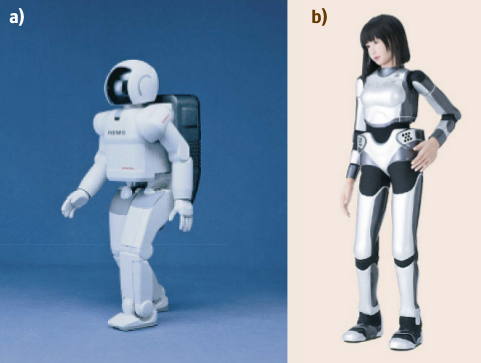
\includegraphics[scale=0.5]{images/asimov_and_HRP-4C.png}
	\caption{Ejemplos de robots humanoides (a) Asimov (2000); (b)HRP-4C (2009). Imagen tomada de: \cite{siciliano2016springer}.}		
\label{fig:humanoids}%(Ver página 423).
\end{figure}


			\subsubsection*{Análisis de estabilidad}

Para el control del sistema dinámico no lineal hay  un número de conceptos relativos para su seguridad y estabilidad:

\begin{itemize}
\item \textit{Puntos fijos} : Representan las posturas estáticas en cuáles el robot puede estar de pie de manera segura.

\item \textit{Ciclos límites}: Proveen una natural extensión del análisis de los puntos fijos para movimientos de caminata periódica.

\item \textit{Viabilidad}: La viabilidad es un concepto de invarianza controlada, que analiza el conjunto de estados del cual el robot es capaz de mantenerse de pie. Desafortunadamente esta propiedad puede ser intratable para el cómputo.

\item \textit{Controlabilidad}: La controlabilidad provee una ligera noción de restricción de viabilidad, analizando el conjunto de estados del cual el robot es capaz de retornar a un particular punto fijo.

\item \textit{Estabilidad robusta}: Examina las propiedades del sistema considerando el "peor de los casos" de las perturbaciones. Por instancias, un controlador robusto debería ser capaz de garantizar que un punto fijo es estable incluso si la estimación de masa del tronco tiene un error del $\pm$10\%.

\item \textit{Estabilidad estocástica}: El análisis estocástico provee herramientas para investigar la probabilidad de caer. Para muchos modelos de perturbaciones en robots el sistema caerá eventualmente (con probabilidad uno), pero el análisis puede revelar la distribución del tiempo de vida metaestable.

\item \textit{Estabilidad de entrada-salida}: En este análisis se trata una particular perturbación como una entrada, un criterio de rendimiento como salida e intenta calcular una ganancia relativa o sensibilidad del rendimiento del robot debido a esta entrada.

\item \textit{Márgenes de estabilidad}: El análisis de robustez puede ser difícil. En la práctica, los diseñadores del control a menudo se conforman con que el sistema se mantenga cómodamente lejos de los límites de estabilidad determinista.		

\end{itemize}

	\section{Aplicaciones en el juego de Futbol Soccer}	
		\subsubsection*{Futbol Soccer en el concurso RoboCup}
		La \textit{RoboCup Federation} es una iniciativa internacional para promover la inteligencia artificial y la tecnología robótica a través de la organización de competencias y encuentros científicos. Una de las categorías más famosas dentro de este concurso es el de fútbol soccer con robots humanoides (Humanoid League) cuyo objetivo es lograr que para la mitad del siglo XXI un equipo de robots humanoides autónomos sean capaces de ganar una partida de fútbol contra el recien campeón mundial de ese entonces, siguiendo las reglas oficiales de la FIFA.
		
		Las competencias de soccer comenzaron en el año de 1997 con simples y simulados robots con ruedas, desde entonces el desarrollo  fue creciendo hasta que en el 2002 se inauguró la liga de humanoides. Para ese entonces los principales retos eran comportamientos como caminar, patear y percibir objetos del ambiente, de esta manera, las mejoras en los mecanismos, la electrónica y control han hecho evolucionar el desarrollo para que la \textit{biomímesis} sea la más parecida a la de un humano.\citep{gerndt2015humanoid}
		
		\subsubsection*{Liga de robots humanoides de categoría \textit{TeenSize}}
		En los recientes años, la introducción de robots estandarizados, accesibles y de bajo costo ha tenido una formidable aceptación para el desarrollo e investigación de robots para soccer. Un ejemplo, es el humanoide \textit{DARwIn-OP} (Figura \ref{fig:Darwin_OP}), este robot cuenta con una plataforma estable, y algunos comportamientos de soccer están ya implementados, de modo que los nuevos desarrolladores tienen la oportunidad de enfocarse en tareas de más alto nivel para hacer los partidos más dinánmicos y complejos. \citep{schwarz2013humanoid}. 
		
		\textit{DARwIn-OP} (categorizado dentro de \textit{KidSize}) ha facilitado que los equipos lleguen a tener el número necesario de jugadores (robots) para los partidos, no obstante, para otras categorías en donde los robots tienden a tener mayor tamaño (\textit{TeenSize} o \textit{AdultSize}) no se llega a tener el número suficiente de jugadores para completar los equipos y algunos competidores se ven forzados a participar con robots hechos por ellos mismos. Consecuentemente esto altera el desempeño de los partidos y retraza el desarrollo de nuevos comportamientos. Para solucionar este problema fue desarrollado un primer prototipo de plataforma abierta basado el \textit{Darwin-OP} para la categoría \textit{TeenSize} llamado \textit{Nimbro-OP} (véase la sección 5.1) el cual tiene un diseño de fácil manufactura, ensamblaje y mantenimiento.	 

\begin{figure}
\centering
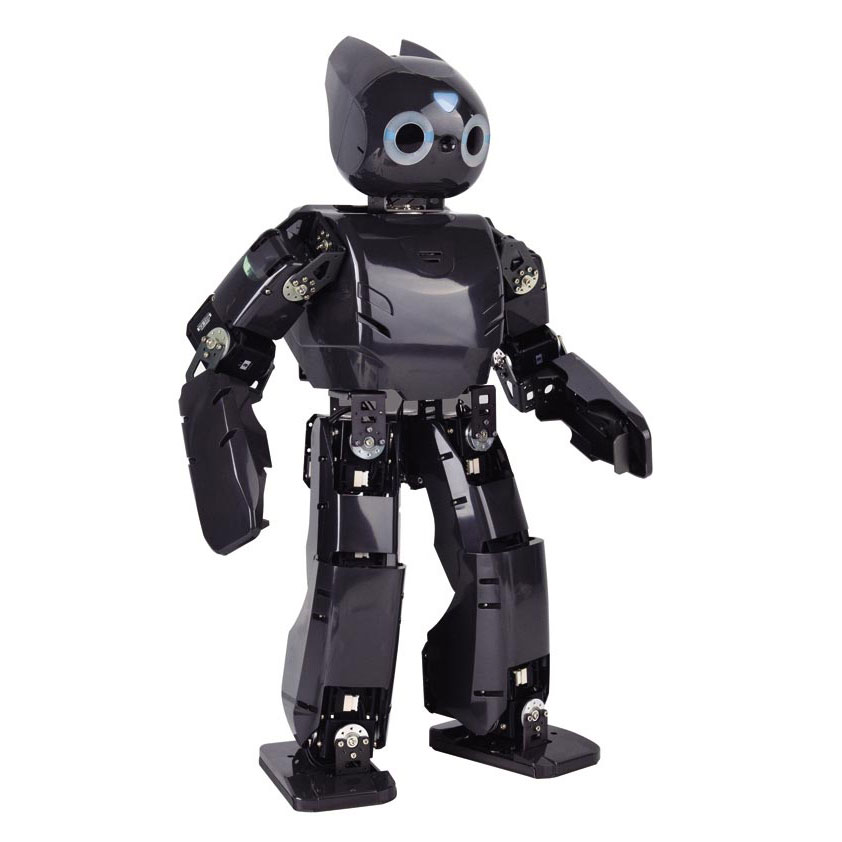
\includegraphics[scale=0.25]{images/Darwin_OP.jpg}
\caption{Robot Humanoide Darwin-OP (Imagen tomada de: http://openrobot.cl/es/robot-darwin-op/).}
\label{fig:Darwin_OP}
\end{figure}

	\section{Usos de la visión computacional}
	La \textit{visión computacional} es la transformación de información lumínica desde una imagen o video a hacia una \textit{nueva representación} de datos \cite{bradski2008learning}. Con esta nueva representación se pueden usar ciertas características de la luz capturada para transformarlas en variables numéricas que la computadora pueda abstraer y procesar (tómese de ejemplo la figura \ref{fig:camera_representation}).

\begin{figure}
\centering
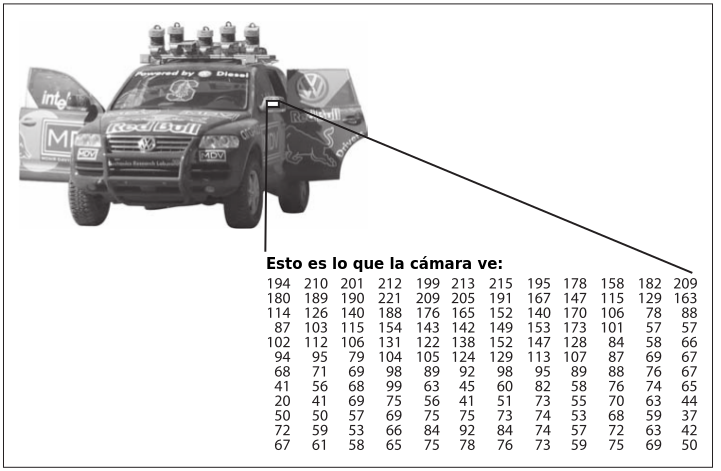
\includegraphics[scale=0.6]{images/new_representation_image.png}
\caption{Representación de cómo una imagen es representada por la computadora. Imagen modificada de: \cite{bradski2008learning}}
\label{fig:camera_representation}
\end{figure}

Para los fines de esta tesis, no es será necesario hacer uso de software para reconocimiento de formas o patrones, solamente se utilizarán funciones para segmentar objetos con base en su color, lo cual es muy conveniente para determinar la posición del objeto en el espacio. Tal y como se puede ver en el análisis matemático de la sección 4.1.
	
	\section{El Filtro de Kalman}
		\subsection*{Filtro de Kalman Discreto}
	En 1060 Rudolf Emil Kalman publicó su famoso \textit{paper} donde describe una forma sencilla para filtrar datos discretos de manera recursiva. Este método ha sido usado ampliamente en investigaciones y aplicaciones de ingeniería ya que resulta útil para la predicción de estados con base en modelos matemáticos y datos estadísticos. Por ejemplo, la posición y velocidad de un avión en vuelo, la temperatura de una caldera a la que se le está suministrando combustible o las lecturas dispersas de posición en un GPS.

	El Filtro de Kalman es un algoritmo computacionalmente eficiente cuyas ecuaciones matemáticas minimizan el error producido por el ruido inherente de las mediciones. Con la estimación es posible conocer con precisión el estado pasado, presente y futuro de un sistema, incluso si éste tiene un modelo de naturaleza desconocida.
	
		\subsection*{Proceso de estimación}
		El Filtro de Kalman aborda el problema de tratar de estimar el estado $x \in \Re^n$ de un proceso de tiempo discreto que es modelado con la ecuación diferencial \ref{eq:kalman_filter}.
		
\begin{equation}
\hat{x}_{n+1,n} = F \hat{x}_{n,n} + G \hat{u}_{n,n}
\label{eq:kalman_filter}
\end{equation}

	En donde $F$ es una matriz de nxn que relaciona el estado presente $n$ con el estado futuro $n+1$. $G$ es una matriz de nx1 que relaciona la entrada de control $u \in R^1$ al estado $x$. 
\\
	La medición $z \in \Re^m$, también conocida como vector de medición se puede modelar con la ecuación \ref{eq:measurement_equation}:

\begin{equation}
z_n = Hx_n+v_n
\label{eq:measurement_equation}
\end{equation}

En donde la matriz de observación $H$ de mxn es la que relaciona el estado $x_n$ con la medición $z_n$, el vector $v_n$ representa el ruido aleatorio en la medición. El Filtro de Kalman supone que el error en las mediciones debe tener una distribución normal, de esta manera la predicción de los estados tendrá un mayor grado de confiabilidad, por lo tanto la expresión \ref{eq:normal_distribution_R} representa cómo está distribuido el error del vector $v_n$. 

\begin{equation}
p(v) \sim N(0,R)
\label{eq:normal_distribution_R}
\end{equation}

Con el objetivo de encontrar una ecuación que calcule la estimación de un estado \textit{a posteriori} $\hat{x}_{n,n}$ como una combinación lineal de un estado \textit{a priori} $\hat{x}_{n, n-1}$ más una proporcional diferencia de la medición actual $z_n$ con la predicción $H\hat{x}_{n,n-1}$ se emplea la ecuación \ref{eq:posteriori_predicted}.

\begin{equation}
\hat{x}_{n,n} = \hat{x}_{n,n-1} + K_n (z_n-H\hat{x}_{n,n-1})
\label{eq:posteriori_predicted}
\end{equation}

$K_n$ es una matriz de nxm llamada \textit{Ganancia de Kalman}, esta ganancia está dada por la ecuación \ref{eq:k_gain} y su valor determina si es más confiable el valor de la medición o la predicción previa del modelo matemático.

\begin{equation}
K_n = P_{n,n-1}H^T(HP_{n,n-1}H^T+R_n)^{-1}
\label{eq:k_gain}
\end{equation}

Como puede observarse, cuando el error de covarianza de la medición $R_n$ se aproxima a cero, la ganancia $K_n$  tiene un mayor peso (cercano a uno). Por el contrario, cuando el error de covarianza \textit{a posteriori} $P_{n,n-1}$ se aproxima a cero, la ganancia $K_n$ obtiene menor peso (cercano a cero).
	La matriz de mxm $Q$ o \textit{matriz de error de proceso} describe el error causado por situaciones imprevistas, causados por ambientes irregulares o fallas mecánicas .	
\\
\\
	El algoritmo consta de dos fases, la fase \textit{predictiva} y la fase \textit{correctiva}. La fase predictiva consta de utilizar un modelo matemático para obtener las probables mediciones de un fenómeno. La fase correctiva obtiene los valores de la medición y las compara con las obtenidas con el modelo matemático, véase la figura \ref{fig:Kalman_scheme}.

\begin{figure}
\centering
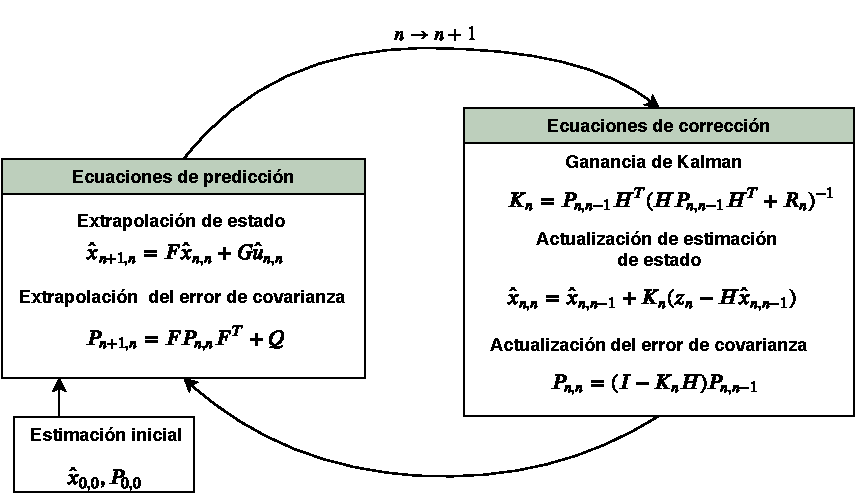
\includegraphics[scale=0.7]{images/kalman_algorithm.pdf}
\caption{Esquema ilustrativo del Filtro de Kalman. Diagrama Modificado de: \cite{welch1995introduction}}
\label{fig:Kalman_scheme}
\end{figure}

	Como ser vio, este filtro utiliza modelos matemáticos lineales, sin embargo en diversas situaciones, el modelo matemático no es lineal, y la predicción resulta ser errónea. Para solucionar esto, se puede implementar el Filtro de Kalman Extendido, que es básicamente el mismo tomando como lineal el modelo en ciertos intervalos de tiempo, y linealizando la predicción de la covarianza del proceso con base en la serie de Taylor. Véase la figura \ref{fig:extended_kalman_scheme}.

\begin{figure}
\centering
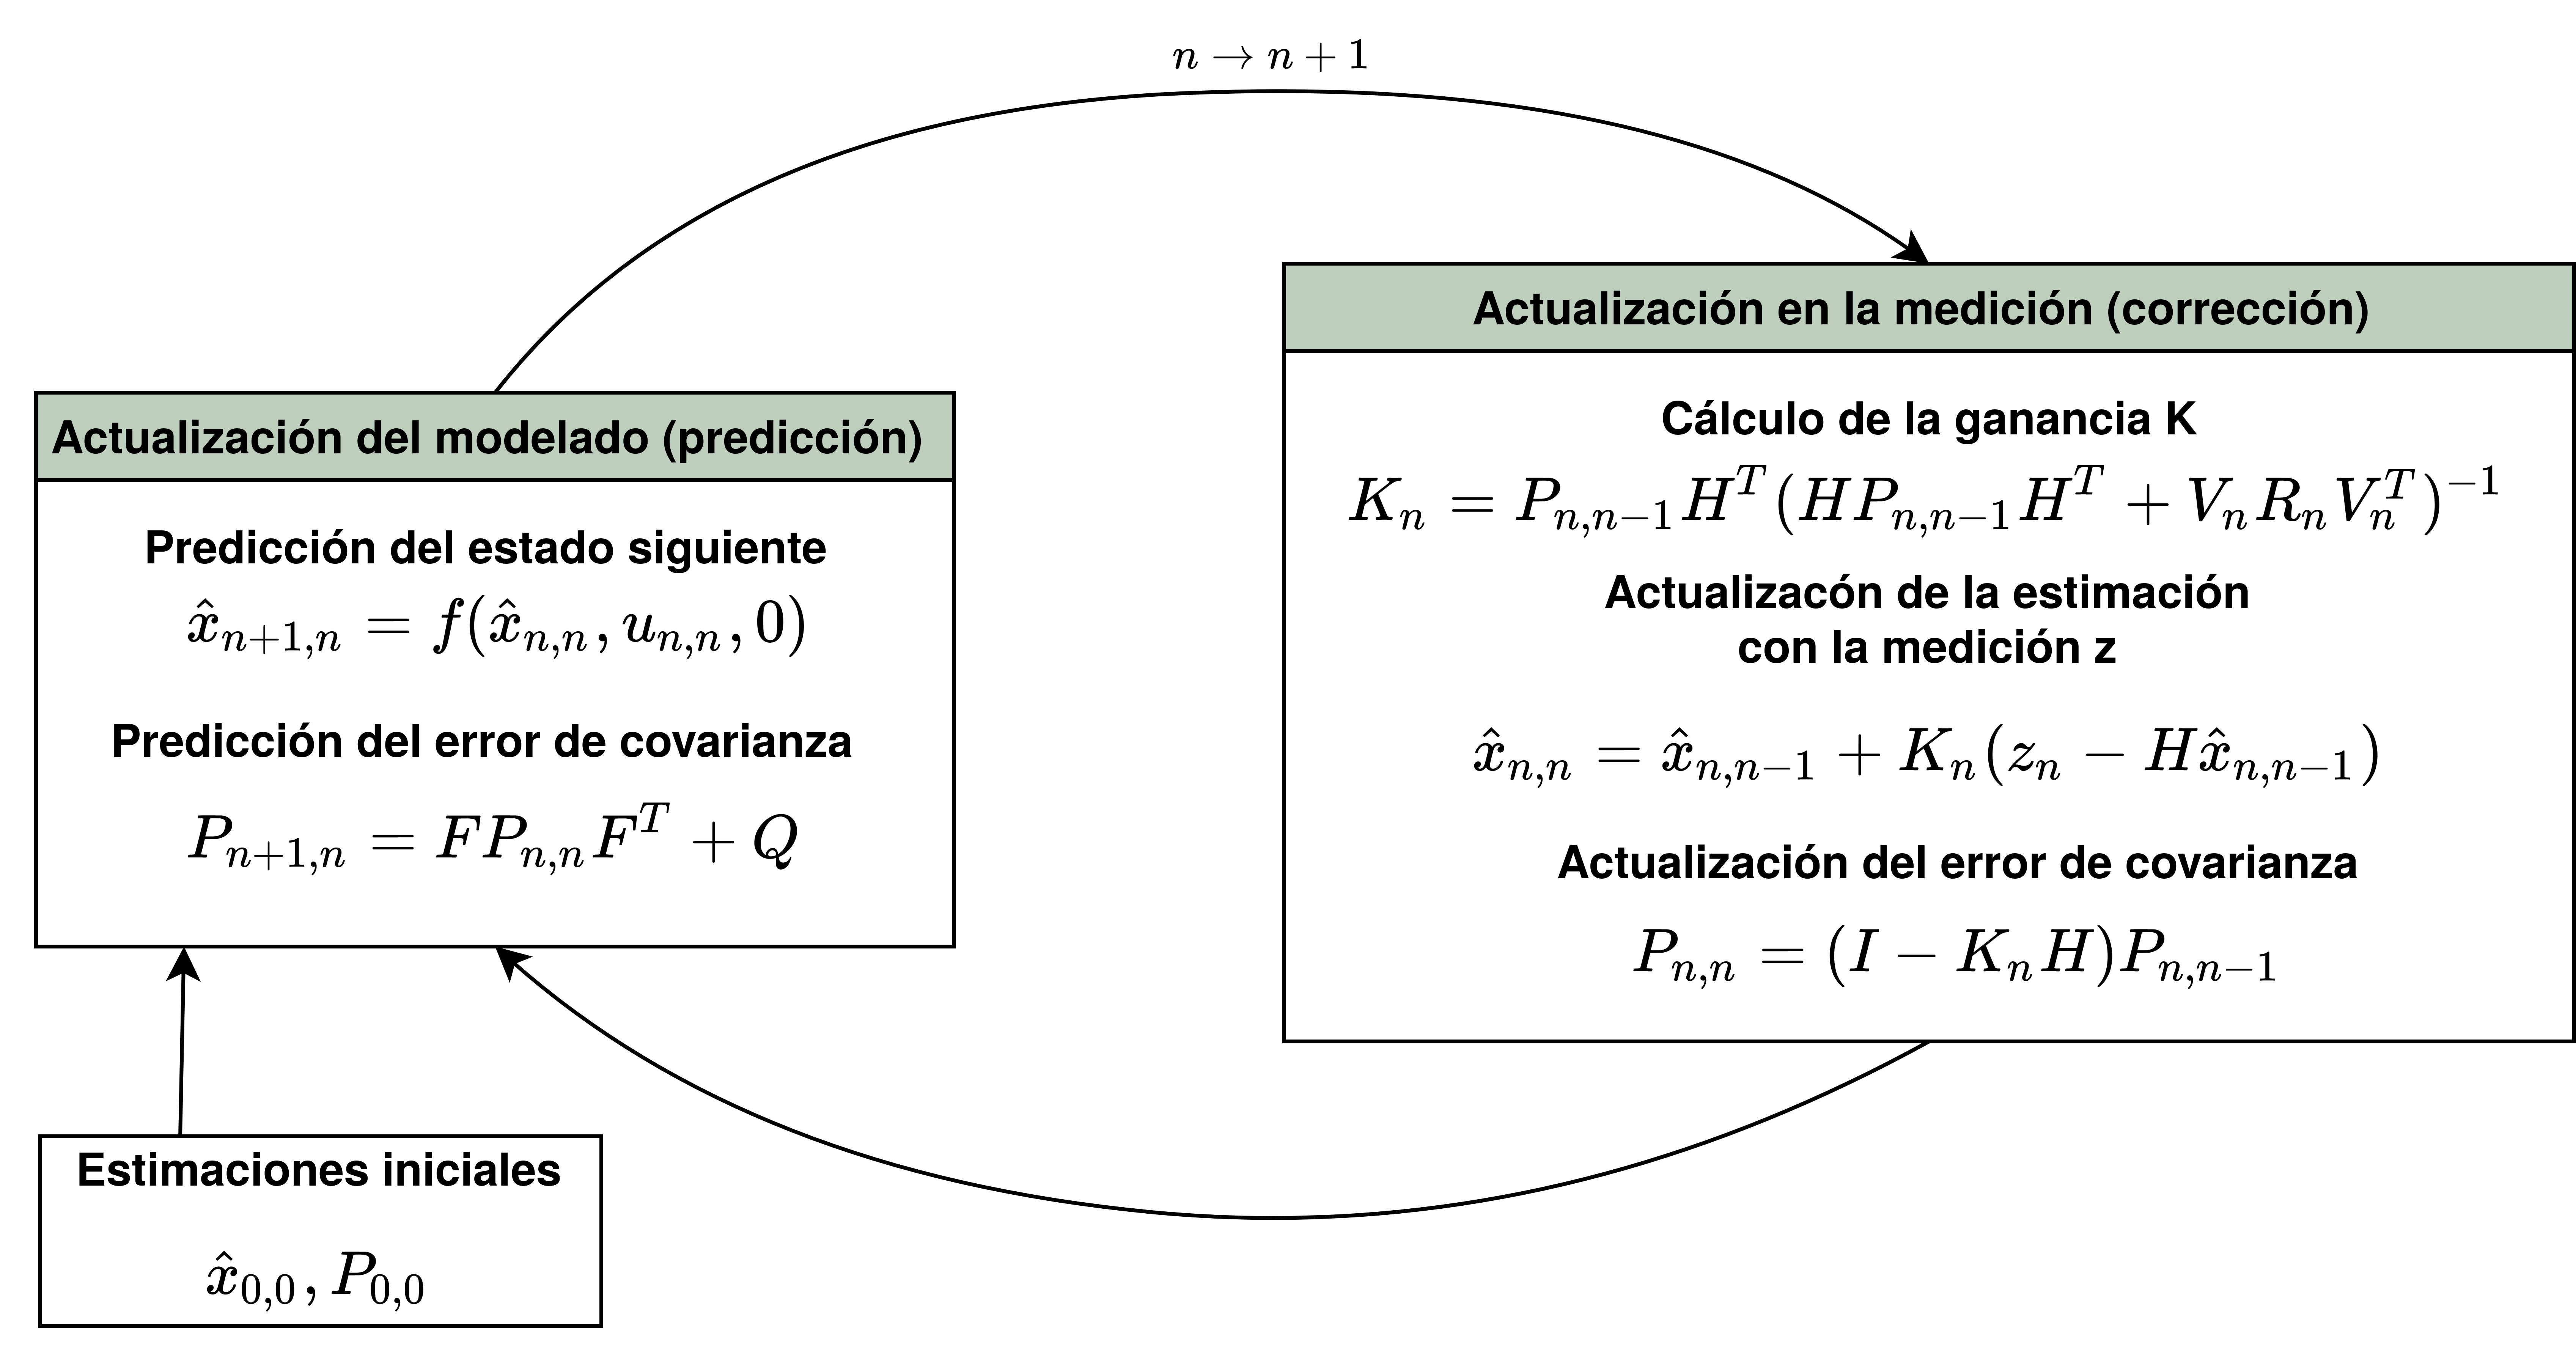
\includegraphics[scale=0.05]{images/extended_kalman_algorithm.png}
\caption{Esquema del Filtro de Kalman Extendido. Diagrama Modificado de: \cite{welch1995introduction}}
\label{fig:extended_kalman_scheme}
\end{figure}

En el capítulo 4 se deduce el modelo matemático del sistema de estimación, y se decide si se trabajará con el filtro extendido o el normal. 
	\section{Trabajo relacionado}
	
	Como ya se ha mencionado, la detección del balón es el principal objetivo para la categoría de \textit{Soccer Humanoids}. Esto representa un reto para los sistemas de visión computacional, el cual debe encargarse tanto de la detección como del cálculo de la posición con base en un sistema egocéntrico. Según los TDP \textit{(Team Description Paper)} se puede saber cómo los equipos han abordado este desafío en los recientes años, por lo que ayuda en gran medida para saber qué técnicas se pueden reimplementar o mejorar según la necesidad. 
\\	

	En los siguientes párrafos se resumen los métodos utilizados por los equipos de distintos países, así será fácil diferenciar con los métodos implementados de esta tesis.
	
	\subsection*{ITAndroids}
	El equipo \textit{ITAndroids} del Instituto Tecnológico de Aereonáutica de Brasil implementó un sistema basado en los sistemas de visión de los humanoides de la plataforma estándar. Tomaron como punto de partida la segmentación por color con algoritmos hechos en MATLAB y funciones de OpenCV como \textit{Hough Circle Transform} para la detección correcta del objetivo, tal y como se ve en la Figura \ref{fig:ITAndroids_vision}.
	
\begin{figure}
\centering
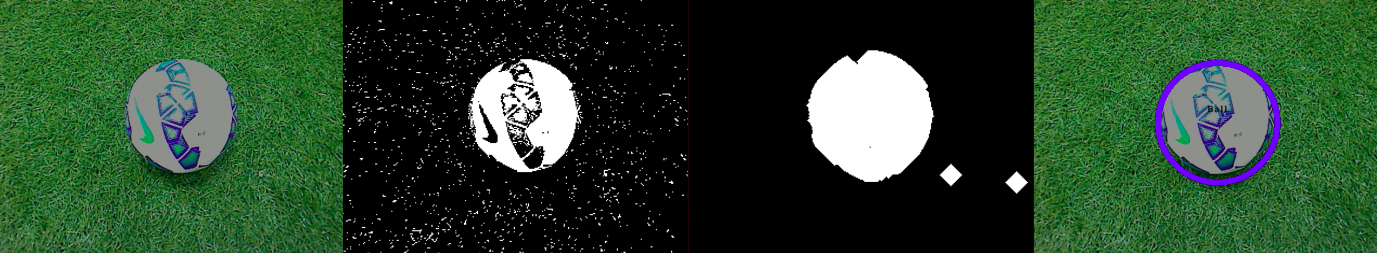
\includegraphics[scale=0.25]{images/ITAndroids_vision.png}
\caption{Proceso de vision implementado por ITAndroids. Imagen tomada de: \cite{davi2017ITAndroids}}
\label{fig:ITAndroids_vision}
\end{figure}

	Debido al ruido inherente en el procesamiento de imágenes, un Filtro de Kalman es empleado para estimar la posición más probable si es que un objeto del mismo color del balón es detectado.
	
	Ya que se hace el reconocimiento del balón, se procede a calcular su posición relativa respecto al humanoide, transformando las coordenadas bidimensionales obtenidas por la imagen a tridimensionales haciendo uso de un método similar al de esta tesis (véase la Sección 4), suponiendo que la posición del balón en la coordenada \textit{z} es siempre 0 y calculando la cinemática directa desde la posición de la cámara a la posición de dicho objetivo.
	
	 \subsection*{NimbRo TeenSize}
	 Debido a las nuevas reglas dadas por el comité organizador de la RoboCup en cuanto al color del balón (blanco como en las competencias de la FIFA), el equipo \textit{NimbRo} de la Universidad de \textit{Friedrich-Wilhelms} de Alemania optó por utilizar un sistema de reconocimiento que no se base sólo en color, pues las líneas divisorias de las canchas o la portería tienen la misma tonalidad. Es por eso que su sistema de reconocimiento está basado en histogramas HOG (histogram of oriented gradients).
	
	 Con el reconocimiento debidamente implementado, se usan las Transformaciones Homogéneas para obtener la posición del balón con cinemática directa, de este modo resulta muy útil la biblioteca \textit{tf2} de ROS. No obstante, aunque las posiciones del robot están bien definidas, algunas variaciones del hardware pueden dar pauta al error en la medición. Para resolver estos fallos este equipo usó el método de Nelder-Mead que consiste en hacer una triangulación convergente para las probables posiciones del balón.
	 
	 \subsection*{T-Flow}
	 Otra forma para realizar la detección de objetos es obteniendo una forma tridimensional específica con una cámara estéreo, tal y como lo hizo el equipo \textit{T-Flow} del \textit{Centro de Investigación de Robótica} del Politécnico de Indonesia. 
	 

	 Este equipo emplea una cámara estéreo para obtener un par de imágenes, remapear y formar una imagen tridimensional con profundidad aproximada, para posteriormente compararse con un patrón esférico como lo es el balón. 	 


	 El sistema de estereo-visión resulta ser muy útil y sencillo para la detección y posicionamiento del objeto, no obstante, se requiere un elevado coste computacional.
	 
	\subsection*{Ichiro}
	De una manera muy similar al robot del Laboratorio de Bio-robótica de la UNAM, los humanoides del equipo \textit{Ichiro} del \textit{Instituto Tecnológico Diez de Noviembre} de Indonesia, poseen una web-cam Logitech C922 con alta definición.
	
	En la detección del balón este equipo emplea un método de Patrones de Binarios Locales el cual es un descriptor de texturas que toma como base la transformación de las imágenes a escala de grises, para posteriormente tomar como contorno los cambios de tonalidad, este método representa bajo costo computacional y hace la segmentación más independiente a los cambios de luz. 
\\

	Como se observó en estos párrafos, existen distintos procedimientos para la detección y localización tridimesional del objeto, las cuales resultan muy prometedoras. No obstante, poco se menciona sobre la detección de objetos en movimiento, y los filtros empleado sólo comprenden modelos estáticos, por lo que esta tesis busca ampliar las fronteras de los algoritmos comunmente empleados. 	 
\chapter{Segmentación de imágenes con base en color}
	\section{Modelo de cámara Estenopeica \textit{(Pinhole)}}

De acuerdo con \cite{bradski2008learning} la visión es la detección de la luz del mundo. El proceso de visión empieza cuando un rayo de luz es emanado desde una fuente hacia un objeto. Cuando la luz choca con el objeto, mucha de esta luz es absorbida, la que no, se puede percibir como el color, de esta manera, la luz reflejada hace su camino hacia el sensor óptico.

El modelo más simple de cómo sucede la captura de luz, es el de la cámara estenopeica o \textit{pinhole}. Una cámara estenopeica se puede imaginar como una habitación sin ventanas en donde la luz únicamente entra por una pequeña apertura en el centro de la pared proyectando así una imagen dentro de la habitación. Véase la Figura(\ref{fig:pinholeCamera}).

\begin{figure}
	\centering		
	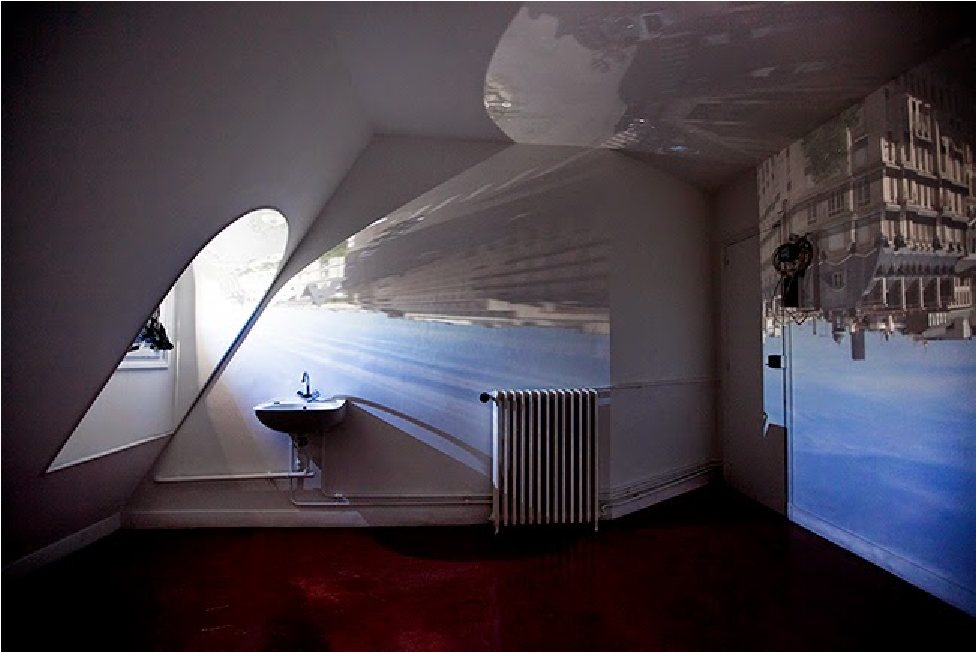
\includegraphics[scale=0.7]{images/pinholeCamera.pdf}
	\caption{Ejemplo en la vida real de la proyección de una imagen con la cámara estenopéica. Imagen tomada de: https://www.pinterest.com.mx/pin/371828512962028619.}		
	\label{fig:pinholeCamera}
\end{figure}

En la cámara estenopeica se considera que sólo un rayo de luz entra desde un punto en particular, este punto es luego \textit{proyectado} sobre una superficie generalmente plana. Como resultado, la imagen en este plano (también llamado plano proyectivo), está siempre en el foco y su tamaño se relaciona a la distancia del objeto por un sólo parámetro: \textit{la distancia focal}. La principal diferencia entre la imagen real y la que aparece en una cámara Pinhole, es que la imagen aparece invertida. 
	
El punto dentro del Pinhole es reinterpretado como el centro de proyección. Para este tipo de cámara, la distancia desde la abertura del Pinhole hacia la pantalla, es precisamente la distancia focal. Como puede verse en la Figura \ref{fig:pinholeScheme}.\\
	
\begin{figure}
	\centering		
	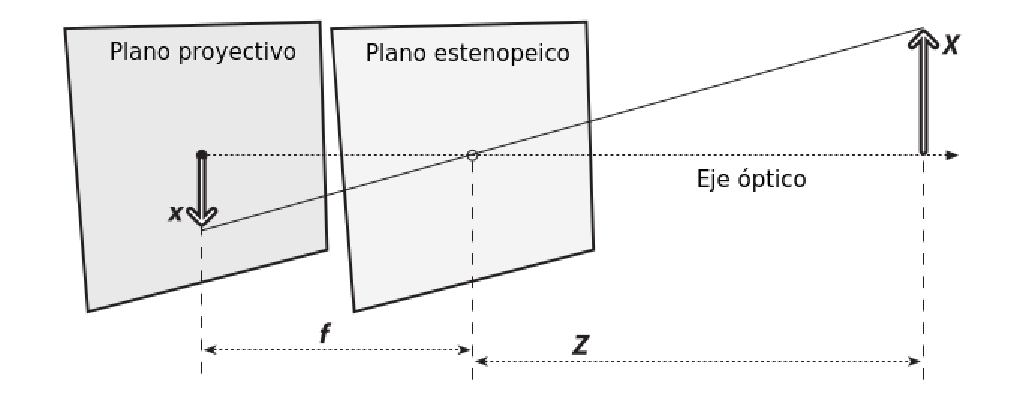
\includegraphics[scale=0.8]{images/pinholeScheme.pdf}
	\caption{Esquema del modelo de cámara estenopeica. Imagen modificada de: \cite{bradski2008learning}.}		
	\label{fig:pinholeScheme}
\end{figure}

En la Figura(\ref{fig:pinholeScheme}), $f$ es representada como la distancia focal de la cámara, $Z$ es la distancia de la cámara al objeto, $X$ es la longitud del objeto, y $x$ es la longitud de la la imagen proyectada en el plano. Dentro de la figura, se pueden ver dos triángulos semejantes de los cuales se puede deducir la siguiente expresión:
\[x = -f \frac{X}{Z}\]
	
Para fines prácticos, el modelo \textit{Pinhole} no es conveniente de usar en exposiciones rápidas, ya que toda su luz proviene de un solo punto. A fin de obtener otro modelo de cámara que recopile mayor cantidad de luz y tenga ecuaciones similares, pero sin signos negativos (correspondientes a la inversión de la imagen) se propone hacer un rearreglo en el que se coloca al frente del centro de proyección el plano proyectivo. Tal y como se ve en la Figura \ref{fig:rearrange_pinhole_scheme}.
	
\begin{figure}
	\centering
	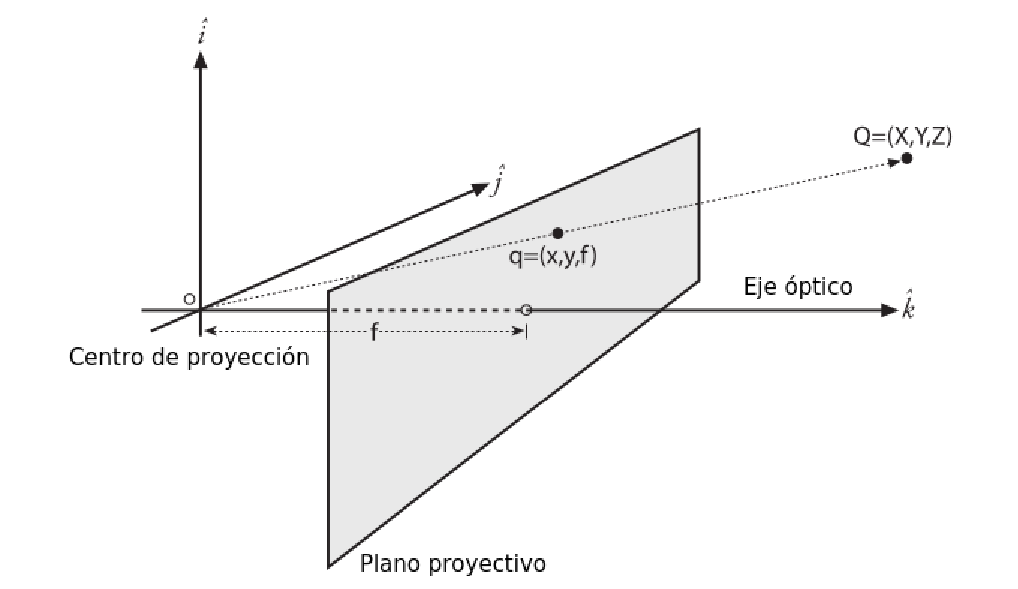
\includegraphics[scale=0.8]{images/rearrange_pinhole_scheme.pdf}
    \caption{Rearreglo de una cámara estenopeica. Imagen modificada de: \cite{bradski2008learning}.}
    \label{fig:rearrange_pinhole_scheme}
\end{figure} 

Con este nuevo cambio, cada rayo de luz proveniente del objeto distante se dirije hacia el \textit{centro de proyección} y deja un punto en el \textit{plano proyectivo}. El punto de intersección del plano proyectivo y el eje óptico es conocido como \textit{el punto principal}. La imagen proyectada en este nuevo plano de imagen, tiene exactamente el mismo tamaño que en el esquema mostrado en la Figura(\ref{fig:pinholeScheme}) pero en este caso, la imagen no queda invertida, por lo que su relación de triángulos quedaría de la siguiente manera: 

\[\frac{x}{f} = \frac{X}{Z}\]

Se podría pensar que que \textit{el punto principal} es equivalente al centro de la imagen, sin embargo, este centro usualmente no está en el eje óptico, es por eso que se introducen dos nuevos parámetros, $c_{x}$ y $c_{y}$ para modelar un posible desplazamiento (perpendicular al eje óptico) del centro de coordenadas en el plano de proyección. El resultado es que un punto $Q$ en el mundo físico cuyas coordenadas son  (X,Y,Z) es proyectado dentro de la pantalla en una localización de pixeles dada por $(x_{screen},y_{screen})$ de acuerdo con las siguientes ecuaciones:

\[x_{screen}=f_{x}\left(\frac{X}{Z}\right ) + c_{x}\]	
\[y_{screen}=f_{y}\left(\frac{Y}{Z}\right ) + c_{y}\]

Nótese que se han introducido dos diferentes distancias focales $f_{x}$ y $f_{y}$, la razón es porque generalmente los pixeles son rectangulares.
		
	\section{Corrección de la distorsión}
		\subsection*{Geometría básica proyectiva}
La relación que mapea los puntos $Q_{i}$ en el mundo físico con coordenadas $(X_{i},Y_{i},Z_{i})$ a los puntos en el plano de proyección con coordenadas $(x_{i},y_{i})$ es llamada una \textit{transformación proyectiva}. Cuando se trabaja con estas transformaciones es conveniente usar las \textit{coordenada homogéneas}. El plano de imagen es el espacio proyectado y tiene dos dimensiones, con lo que se pueden representar puntos en el plano como un vector tridimensional $q=(q_{1},q_{2},q_{3})$ ó $q=(x, y, w)$, en donde w es la orientación. Una forma de hacer un arreglo con los parámetros que definen a la cámara $f_{x},f_{y},c_{x}$ y $c_{y}$ dentro de una matriz de 3x3 es la llamada \textit{matriz de parámetros intrínsecos}. La proyección $q$ de los puntos del mundo físico en el plano de la imagen se puede calcular como: 
\[q=MQ\]
donde
\[q=
\begin{bmatrix}
x\\ 
y\\
w 
\end{bmatrix}\;,\;M=
\begin{bmatrix}
f_{x} & 0 & c_{x}\\ 
0     &f_{y}&c_{y} \\
0     & 0 & 1
\end{bmatrix}\;,\;Q=
\begin{bmatrix}
X\\
Y\\
Z
\end{bmatrix}
\]
		\subsection*{Distorsión de las lentes}
Debido a diversos factores en la manufactura, las lentes de una cámara no son perfectas, y al obtener una imagen, esta puede notarse distorsionada (véase la Figura \ref{fig:image_distorted}). La distorsión es un fenómeno que todas las cámaras tienen, no obstante, es más evidente en las cámaras de baja calidad o en las que tienen lentes tipo \textit{ojo de pescado}. Las distorsiones más características son: las \textit{Distorsiones radiales} y las \textit{Distorsiones tangenciales}. Las primeras surgen como resultado de la forma de las lentes y las segundas como resultado del proceso de ensamblado de la cámara.

\begin{figure}
\centering
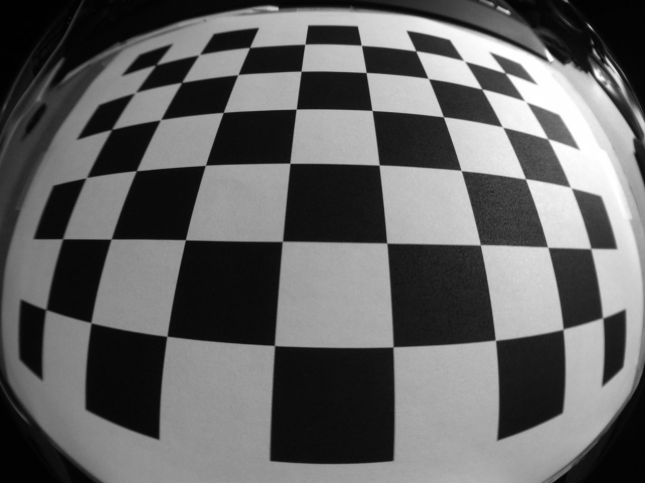
\includegraphics[scale=0.5]{images/image_distorted.png}
\caption{Ejemplo de distorsión de una cámara. Imagen tomada de: https://answers.opencv.org/question/114056/chessboard-detection-fails-on-fisheye-image/?sort=votes}
\label{fig:image_distorted}
\end{figure}

Cuando la imagen se hace más pequeña conforme está más cerca de los bordes se está viendo una \textit{distorsión radial} (véase la figura \ref{fig:radial_distortion}). En la práctica, se puede caracterizar con la serie de Taylor, las ecuaciones son:
\[x_{corregida} = x(1+k_1r^2+k_2r^4+k_3r^6)\]
\[y_{corregida} = y(1+k_1r^2+k_2r^4+k_3r^6)\]

En donde $(x,y)$ son las coordenadas de la imagen, \textit{r} es la distancia del punto de la imagen al centro y las constantes $k_1$, $k_2$ y $k_3$ son parámetros que están relacionados a cada cámara en específico.

\begin{figure}
\centering
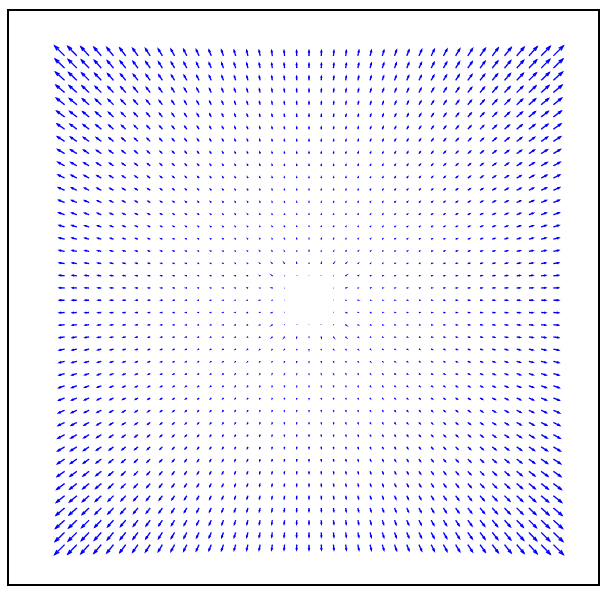
\includegraphics[scale=0.75]{images/radial_distortion.png}
\caption{Distribución de la distorsión radial de una imagen. Imagen tomada de: https://www.i-ciencias.com/pregunta/96683/que-es-el-tangencial-distorsion-de-opencv-en-realidad-tangencial .}
\label{fig:radial_distortion}
\end{figure}

Las \textit{Distorsiones tangenciales} son ocasionadas por no tener paralelas las lentes con el plano de la imagen, vea la distribución de la distorsión tangencial en la figura \ref{fig:tangential_distortion}. Para obtener expresiones que ayuden a corregir este tipo de distorsión se introducen dos parámetros: $p_{1}$ y $p_{2}$ dentro de las siguientes ecuaciones:
\[x_{corregida} = x + [2p_1y+p_2(r^2+2x^2)]\]
\[y_{corregida} = y + [p_1(r^2+2y^2)+2p_2x]\]

La estimación de los parámetros internos es importante en la calibración de las cámaras, de esto depende la exactitud de las mediciones de distancia dadas por la visión computacional. \cite{bradski2008learning}.

\begin{figure}
\centering
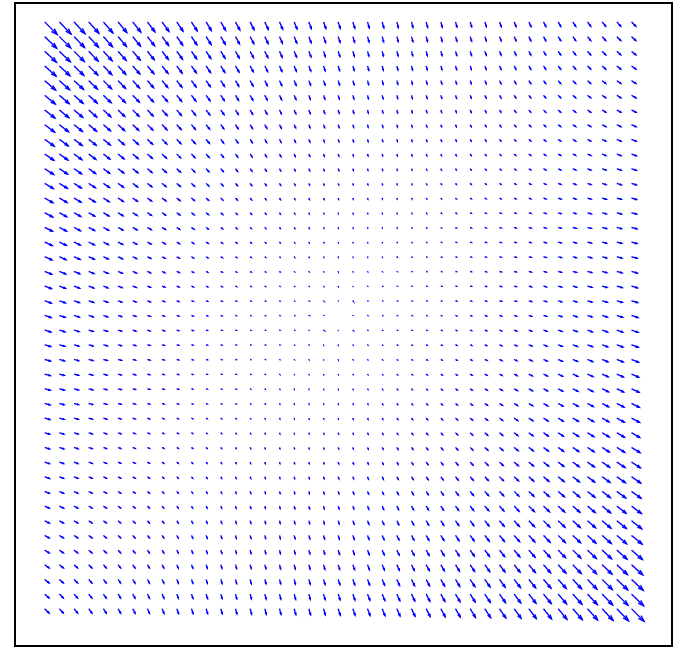
\includegraphics[scale=0.66]{images/tangential_distortion.png}
\caption{Distribución de la distorsión tangencial en una imagen. Imagen tomada de: https://www.i-ciencias.com/pregunta/96683/que-es-el-tangencial-distorsion-de-opencv-en-realidad-tangencial .}
\label{fig:tangential_distortion}
\end{figure}

Para poder hacer una corrección automática de todas las distorsiones, las herramientas de OpenCV (véase la sección 5.2) usan los cinco parámetros antes mencionados dentro de una matriz de 1x5 llamada \textit{matriz de coeficientes de distorsión}, en donde cada parámetro se acomoda de la siguiente forma:
\[[k_1 \quad k_2 \quad p_1 \quad p_2 \quad k_3]\]
	\section{Los espacios de color RGB y HSV}
El el pocesamiento de imágenes se usa el color debido a que es un buen descriptor para la identificación de objetos (mejor que otro tipo de segementación como el de escala de grises) \cite{gonzalez2002digital}.
		\subsection*{Percepción del color}
Según \cite{agoston2005computer} en el caso más simple, la percepción del color tiene tres características principales llamadas \textit{matiz, saturación y brillo}. 
\begin{itemize}
\item \textit{Matiz (Hue):} La matiz es un descriptor de qué tan combinados están los colores unitarios entre sí (si se entiende por color unitario a los colores rojo, amarillo, verde y azul).

\item \textit{Saturación (Saturation): } La saturación es la percepción de la relativa carga de color que tiene la matiz. Se puede decir que la saturación es una medida de qué tan puro es un color si éste es diluido en blanco.

\item \textit{Brillo: (Brightness)} El brillo es un atributo de la iluminación en la cual un objeto no aislado se ve afectado, es notable cuando un objeto de un  mismo color cambia su tonalidad debido a las variaciones de iluminación de su entorno.
\end{itemize}
		\subsection*{Espacios de color}
El \textit{espacio de color} es un modelo utilizado para facilitar la especificación de cualquier color de una manera estandarizada. Uno de los sistemas más conocidos, es el espacio de color RGB (por sus siglas en inglés red, green y blue), que está basado en un sistema coordenado ortogonal (como se observa en la Figura 2.3) en donde la escala de los colores primarios está cada uno en los ejes.

El espacio de color \textit{HSV (Hue-Saturation-Value)} es especificado por tres números que corresponden a la matiz (Hue), saturación (saturation) y el valor (value). La matiz corresponde a un ángulo de 0 a 360 grados. La saturación se toma entre valores de 0 a 1 que miden la salida de la matiz del blanco. El valor (value) que va del 0 al 1 mide la salida de la matiz del negro o \textit{color de energía cero}, véase la Figura 2.4 en donde se observa el modelo tridimencional de este espacio.

\begin{figure}
	\centering		
	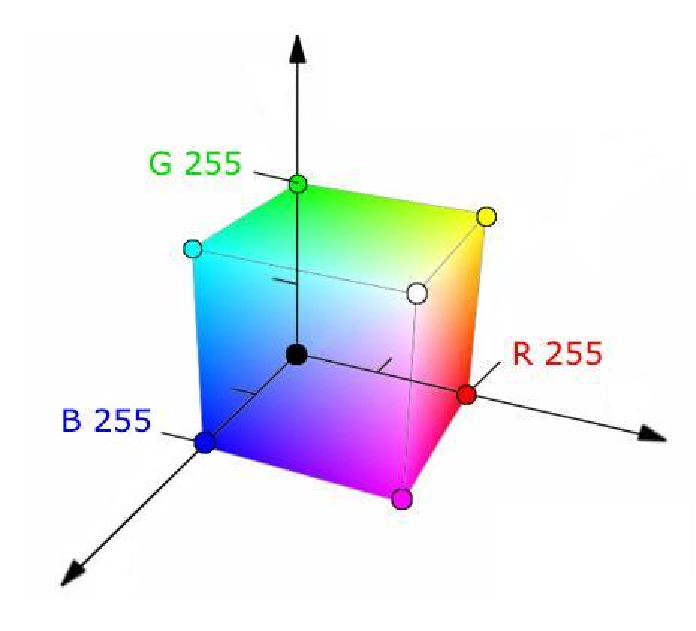
\includegraphics[scale=0.8]{images/RGB_model.pdf}
	\caption{Modelo tridimensional del espacio de color RGB. Imagen tomada de: https://lpurpura.wordpress.com/2011/05/03/modo-de-color/ .}		
\end{figure}

\begin{figure}
	\centering		
	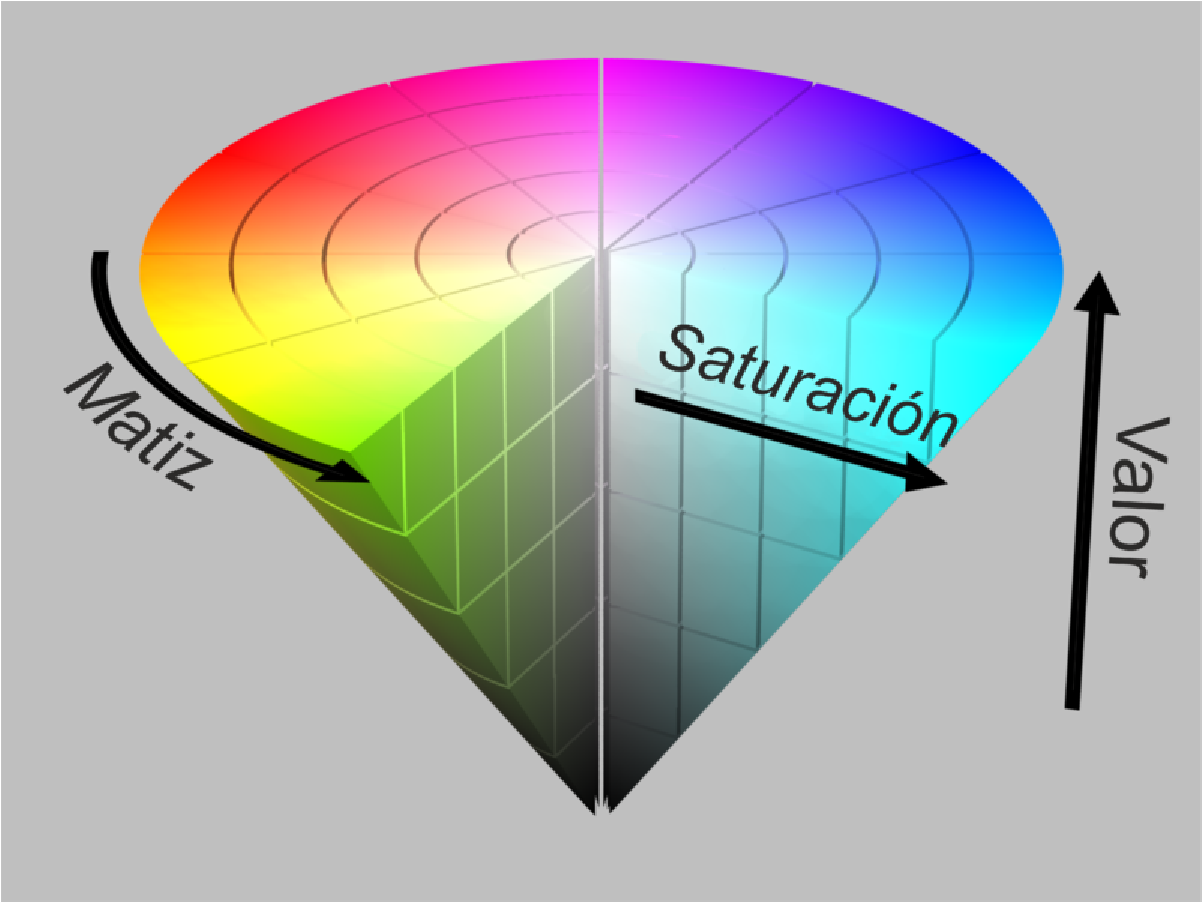
\includegraphics[scale=0.4]{images/hsv_space.pdf}
	\caption{Modelo tridimensional del espacio de color HSV. Imagen tomada de: $https://es.wikipedia.org/wiki/Modelo_-de_-color_-HSV$ .}		
\end{figure}

Tanto el espacio de color RGB y el HSV pueden representar la totalidad de los colores del espectro de luz visible, no obstante para el procesamiento de imágenes se utiliza el HSV ya que es una forma más sencilla para segmentar colores y es una forma más parecida a la que los seres humanos percibimos los colores.

	\section{Operadores morfológicos}	
La gran mayoría de las veces, cuando se hace procesamiento de imágenes, se necesitan ciertos procesos para eliminar el ruido circundante y dejar al elemento de interés aislado. Los \textit{operadores morfológicos} (erosión y dilatación) se pueden usar para este propósito.

Los \textit{operadores morfológicos} son operadores matemáticos basados en la forma de una imagen comunmente binaria (con pixeles blancos y negros) y sirven para preservar sus características y eliminar las irrelevancias. Dado que toda imagen está compuesta por pixeles, se pueden crear ciertos conjuntos de pixeles dentro de un vector para así poder aplicar operaciones matemáticas. 

La \textit{erosión} es el primer operador que se aplica cuando se desea eliminar el ruido en una segmentación, eso es porque elimina una gran cantidad de pixeles que tienden a tener mucha menor área que la figura de interés. Para lograr esto se establecen dos conjutos (de coordenadas de pixeles) $A$ y $B$. Si $A$ y $B$ son conjuntos dentro de un espacio euclidiano de N elementos, entonces la erosión de $A$ por $B$ es el conjunto de elementos $x$ para el cual $x + b \in  A$ para cada $b \in B$. Por lo tanto, de una manera más formal, la operación de erosión se puede definir con la expresión \ref{eq:erosion}.
En la figura \ref{fig:erosion_diagram} se puede observar de una manera más visual cómo funciona la operación de erosión dentro de una imagen binaria.
\begin{equation}
A\thinspace\ominus\thinspace B\thinspace=\thinspace \left \{ x \in E^N  \mid x+b \in A \enspace \forall \; b \in B\right \}
\label{eq:erosion}
\end{equation}

 Para entender de mejor manera cómo es esta operación se debe entender lo que es un \textit{kernel}. Un \textit{kernel} es un conjunto de pixeles de cualquier forma o tamaño que se caracteriza por tener un pixel de anclaje dentro de sí (en la figura \ref{fig:erosion_diagram} es el pixel con un punto blanco). En el ejemplo de la figura \ref{fig:erosion_diagram} se le llamará \textit{kernel} al conjunto $B$ y siempre debe ser de menor tamaño que el conjuto $A$. La intersección del conjunto $A$ con el $B$ al ir colocando el pixel de anclaje en cada pixel del conjunto $A$ es la imagen resultante para la erosión.
 
\begin{figure}
\centering 
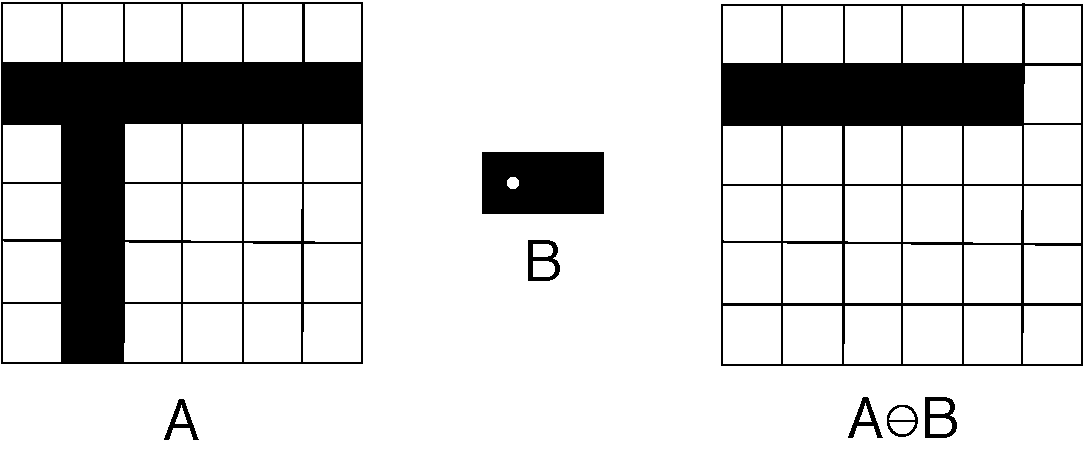
\includegraphics[scale=0.7]{images/erosion_diagram.pdf}
\caption{Ejemplo de la operación de erosión en una imagen binaria.}
\label{fig:erosion_diagram}
\end{figure}

En la figura \ref{fig:erosion_example} se ve que la erosión ha eliminado el ruido y la imagen se ve más limpia de puntos blancos que rodean la región de interés. El problema de hacer este procedimiento es que la imagen original suele verse afectada y tiende a encogerse o a deformarse, esto puede representar un problema para la detección de contornos. Para solucionarlo se procede a aplicar una operación opuesta a la erosión, mejor conocida como \textit{dilatación}.

Una vez eliminado el ruido gracias a la erosión, la \textit{dilatación} procede a ensanchar la figura de interés utilizando la adición de dos conjuntos de elementos. De la misma manera en que se hizo la erosión se procede a nombrar dos conjuntos $A$ y $B$. Si $A$ y $B$ son conjuntos dentro de un espacio euclidiano de N elementos. Sean $a \in A$ y $b \in B$ en donde $a=(a_1, ... ,a_n)$ y $b=(b_1,...,b_n)$, es decir conjuntos con coordenadas de pixeles, entonces la dilatación de $A$ por $B$ es el conjunto de todas las posibles sumas de elementos, de $A$ y $B$. De forma formal se expresa como \ref{eq: dilation}.
\begin{equation}
A\thinspace\oplus\thinspace B\thinspace=\thinspace \left \{ c \in E^N  \mid c=a+b \quad\forall \quad a \in A \; y\; \; b \in B\right \}
\label{eq: dilation}
\end{equation}


\begin{figure}
\centering
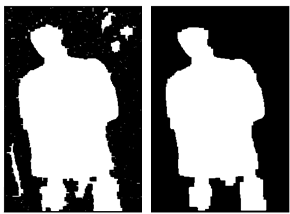
\includegraphics[scale=1]{images/erosion_example.png}
\caption{Eliminación de ruido alrededor de una figura de interés usando la erosión.  Imagen tomada de: $https://docs.opencv.org/3.4/d9/d61/tutorial_-py_-morphological_-ops.html$ .}
\label{fig:erosion_example}
\end{figure}

En la figura \ref{fig:dilation_diagram} se puede imaginar que si se coloca el \textit{kernel} dentro de los pixeles pertenecientes al conjunto $A$ y se suman, queda como resultado de $A \oplus B$ una imagen ensanchada, lo que puede ayudar a que la figura erosionada tenga mayor parecido a la imagen original \cite{4767941}. En la figura \ref{fig:dilation_example} está un ejemplo de cómo se ensancha una figura al aplicar la dilatación.

\begin{figure}
\centering
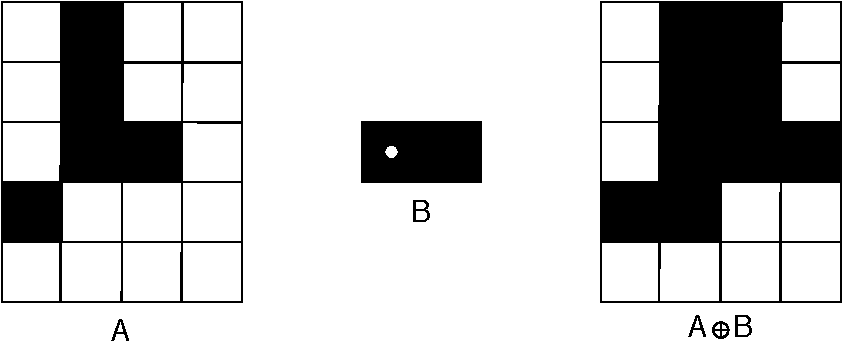
\includegraphics[scale=1]{images/dilation_diagram.pdf}
\caption{Ejemplificacion de la operación de dilatación en una imagen binaria.}
\label{fig:dilation_diagram}
\end{figure}

\begin{figure}
\centering

\includegraphics[scale=0.7]{images/dilation_example.jpg}
\caption{Ejemplificación de la dilatación aplicada en una segmentación de color. Imagen tomada de: $https://unipython.com/segmentacion-imagenes-algoritmo-watershed/$ .}
\label{fig:dilation_example}
\end{figure}
\chapter{Estimación de posición y velocidad}
	\section{Cálculo de la posición del objeto de interés}
Tal como se observa en la simulación de Gazebo (Figura 3.1), se decidió usar un sistema ortogonal derecho en la base de los pies como sistema de referencia que gobernará a todo el modelo.

\begin{figure}
	\centering		
	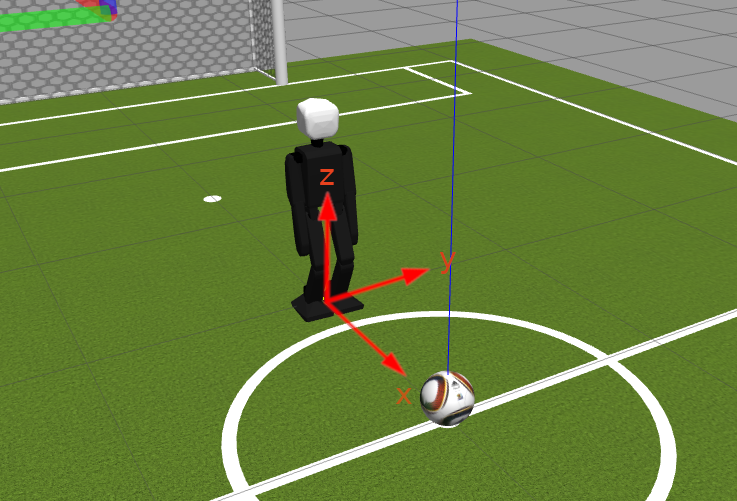
\includegraphics[scale=2]{images/robot_ejes.png}
	\caption{Representación del sistema de referencia usado en el robot.}		
\end{figure}

La cámara está localizada en la cabeza del humanoide, por lo que su centro
de visión se puede representar por un eje que va de la cámara al centroide del 
objeto, en este caso un balón de fútbol.
Para estimar la posición de un objeto que cruce por el centro de visión de la
cámara se necesita establecer un vector unitario:
\[\hat{u} = (u_x, u_y, u_z)\]
conocido en computación gráfica como vector \textit{look at}, (ver figura \ref{fig:LookAt}). Para obtener la ecuación vectorial de la recta paralela al vector \textit{look at} se toma un punto que contenga la recta, en este caso la posición de la cabeza en donde se encuentra la cámara: 

\begin{figure}
	\centering		
	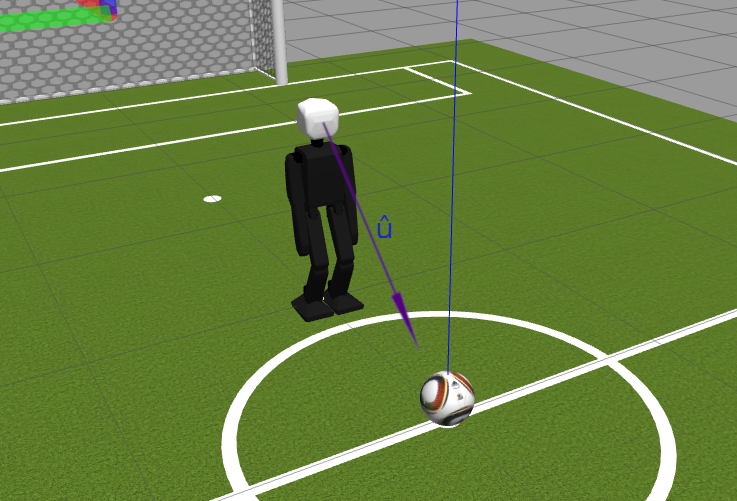
\includegraphics[scale=2]{images/robot_lookat.png}
	\caption{Representación del vector \textit{look at} utilizado en visión computacional.}		
	\label{fig:LookAt}
\end{figure}

\begin{equation}
\label{eq:LookAt}
r(\lambda) = (r_x, r_y, r_z)\quad +\quad \lambda (u_x, u_y, u_z)
\end{equation}


En donde $(r_x, r_y, r_z)$ es la posición en el espacio de la cámara utilizada, referida al sistema de referencia anteriormente mencionado. Se considera que el objetivo siempre estará en el suelo, por lo que el punto de intersección de la ecuación de la recta con el suelo hacen que la variable de altura sea igual a cero, conforme a la siguiente expresión:
\[r = (x, y, 0) = (r_x, r_y, r_z) + \lambda (u_x, u_y, u_z)\]
Despejando $\lambda$ del tercer término de la expresión anterior se obtiene:
\[\lambda = -\frac{r_z}{u_z}\]

De esta manera, substituyendo $\lambda$ en (\ref{eq:LookAt}), se obtiene:
\[x = r_x-\frac{r_z u_x}{u_z}\]
\[y = r_y-\frac{r_z u_y}{u_z}\]

Ya teniendo estas expresiones se procede a sustituir al vector unitario \textit{look at} con coordenadas esféricas, tal y como se observa en la siguiente expresión:
\begin{equation}
\label{eq:LookAtUnitary}
\hat{u}=(u_x, u_y, u_z)=(\sin{ \theta}\cos{\varphi},\sin{\theta}\sin{ \varphi},\cos{\theta})
\end{equation}

Sustituyendo la expresión (\ref{eq:LookAtUnitary}) dentro de los valores $x$ y $y$ da como resultado:
\[x=r_x - \frac{r_z \sin{ \theta} \cos{\varphi}}{\cos{\theta}}\]
\[y=r_y - \frac{r_z \sin{\theta} \sin{ \varphi}}{\cos{\theta}}\]

Utilizando la identidad trigonométrica:
\[\tan{\theta} = \frac{\sin{\theta}}{\cos{\theta}}\]

Las ecuaciones para obtener la posición del objetivo siempre y cuando $z=0$ son:
\begin{equation}
\label{eq:xBidimentionalPosition}
x=r_x - r_z \tan{\theta}  \cos{\varphi}
\end{equation}

\begin{equation}
\label{eq:yBidimentionalPosition}
y=r_y - r_z \tan{\theta} \sin{\varphi}
\end{equation}

No obstante, el objeto a considerar no es un objeto bidimensional, es un balón con forma esférica que está sobre el plano del suelo, debido a esto se pueden complementar las ecuaciones \ref{eq:xBidimentionalPosition} y \ref{eq:yBidimentionalPosition}, para obtener la posición (x,y,z) del centro del balón.

En la figura \ref{fig:ballProjection}(a) se observa un diagrama del balón en donde el vector \textit{look at} atravieza su centro e intersecta con el suelo en un punto en donde el balón no está. Esto representa un problema, ya que la posición en $x$ sufre una proyección, la cual incrementa mientras el balón tenga mayor radio. A esta proyección se le pondrá la variable $x_c$. Véase la figura \ref{fig:ballProjection}(b)


\begin{figure}
	\centering
	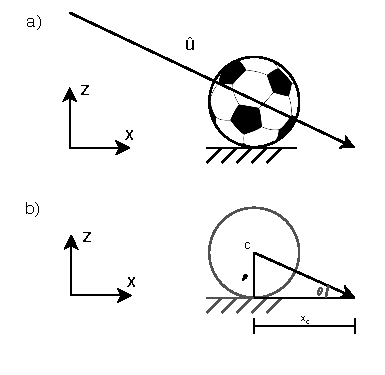
\includegraphics[scale=1.4]{images/ball_projection.pdf}
	\caption{(a) Bosquejo del vector \textit{look at} atravezando el centro del balón esférico; (b) Diagrama de la obtención de la distancia de proyección $x_c$.}
	\label{fig:ballProjection}
\end{figure}

Para obtener la magnitud de $x_c$ es necesario analizar el diagrama de la figura \ref{fig:ballProjection}(b), en donde $\theta$ es el ángulo \textit{pitch} y $\rho$ es el radio del balón. Así se puede obtener la siguiente igualdad:
\[\cot{\theta} = \frac{x_c}{\rho}\]\\

Despejando $x_c$
\[x_c = \rho \cot{\theta}\]

Debido a que $x_c$ se ve afectada también por la posición \textit{yaw} se deducen las siguientes igualdades para corregir el valor de la posición de $x$ y $y$ respectivamente:

\begin{equation}
\label{eq:xcForX}
x_{cx} = \rho \cot{\theta} \cos{\varphi}
\end{equation}

\begin{equation}
\label{eq:xcForY}
x_{cy} = \rho \cot{\theta} \sin{\varphi}
\end{equation}\\

De esta manera, se resta \ref{eq:xcForX}  a \ref{eq:xBidimentionalPosition} y \ref{eq:xcForY} a \ref{eq:yBidimentionalPosition}. Finalmente las ecuaciones resultantes son:

\[x = r_x - r_z \tan{\theta} \cos{\varphi} - \rho \cot{\theta} \cos{\varphi}\]
\[y = r_y - r_z \tan{\theta} \sin{\varphi} - \rho \cot{\theta} \sin{\varphi}\]
\[z = \rho \]


		
	\section{Estimación de estados mediante el Filtro de Kalman}
	Para poder impementar el Filtro de Kalman, se necesita primero tener un modelo matemático del sistema que se pretende tomar mediciones. Analizando el digrama de cuerpo libre de la Figura \ref{fig:dynamic_model} se puede hacer un análisis dinámico del balón utilizando la segunda ley de Newton.

\begin{equation}
\sum F = m \ddot{x}
\label{eq:second_law}
\end{equation}

\begin{equation}
F-f_{fricción} = m \ddot{x}
\label{eq:equivalency_1}
\end{equation}

Cambiando el nombre de las variables a corde de nuestro diagrama y tomando en como fuerza de fricción dinámica $f_{fricción} = \mu_d m g $ la igualdad de fuerzas es:
\begin{equation}
F- \mu_d m g = m  \frac{\mathrm{d} \dot{x}}{\mathrm{d} t}
\label{eq:equivalency_2}
\end{equation}
	
Donde $\mu_d$ es el coeficiente de fricción dinámica, $m$ es la masa del balón y $g$ es la aceleración de la gravedad. Debido a que la fuerza de fricción es la única que actúa sobre el balón, $F$ se iguala a cero, dejando el modelo el modelo cinemático de la expresión \ref{eq:mathematical_model_1}.

\begin{equation}
\frac{\mathrm{d} \dot{x}}{\mathrm{d} t} = - \mu_d g
\label{eq:mathematical_model_1}
\end{equation}

Despejando la variable $\dot{x}$ para se puede integrar la ecuación para obtener la velocidad en el tiempo $t$ del balón.
\begin{equation}
\int_{\dot{x}_0}^{\dot{x}} \mathrm{d} \dot{x} = -\mu_d g \int_{0}^{t} \mathrm{dt}  
\label{eq:mathematical_model_2}
\end{equation}

Resolviendo la ecuacion \ref{eq:mathematical_model_2} y despejando $\dot{x}$ se puede obtener la siguiente expresión:
\begin{equation}
\dot{x} = \dot{x}_{0} - \mu_d g t 
\label{eq:velocity_prediction}
\end{equation}

Una vez teniendo el modelo para predecir la velocidad del estado siguiente, se procede a integrar nuevamente para obtener su posición:
\begin{equation}
\int_{x_{0}}^{x} \mathrm{dx} = \int_{0}^{t} (\dot{x}_{0} - \mu_d g t) \mathrm{dt}
\label{eq:mathematical_model_4}
\end{equation}

Integrando y despejando $x$ se obtiene:
\begin{equation}
x = x_0 + \dot{x}_0 t - \frac{1}{2} \mu_d g t^2
\label{eq:position_prediction}
\end{equation}

%ESta ecuación es la solución de la ecuación diferencial que modela el movimiento
%De la eacuación 4.9 se tiene que:
Ya obtenida la ecuación para obtener la posición, despejamos la aceleración del modelo \ref{eq:equivalency_2}:
\begin{equation}
\ddot{x} = -\frac{1}{m}\mu_d m g + \frac{1}{m}F
\end{equation}

Pero F = 0. Es decir, que simplemente el balón comienza con $v_{0}$ diferente de cero y se va deteniendo.
Planteando esto en variables de estado:
\[ [x_1,x_2] = [x, \dot{x}]\]

En donde:
%\begin{eqnarray*}
\begin{equation}
\dot{x}_1 = x_2
\label{eq:state_variable_1}
\end{equation}

\begin{equation}
\dot{x}_2 = -\frac{1}{m}\mu_d m g + \frac{1}{m}F
\label{eq:state_variable_2}
\end{equation}

%\end{eqnarray*}

\begin{figure}
\centering
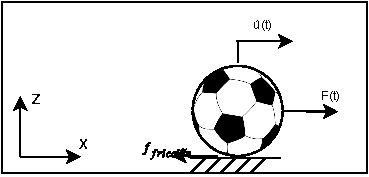
\includegraphics[scale=1.5]{images/dynamic_model.pdf}
\caption{Diagrama de cuerpo libre del objeto de interés}
\label{fig:dynamic_model}
\end{figure}

		\subsubsection*{Descripción del proceso de filtrado en el sistema}
Con el modelo dinámico que describe el movimiento del balón, se procede a escribir las ecuaciones matriciales del Filtro de Kalman (Véase la sección 2.4). De este modo, este filtro es una serie de pasos que iterativamente se deben ir completando para estimar posiciones y velocidades de un objeto en movimiento (Figura: \ref{fig:kalman_extended_diagram}).

\begin{figure}
\centering
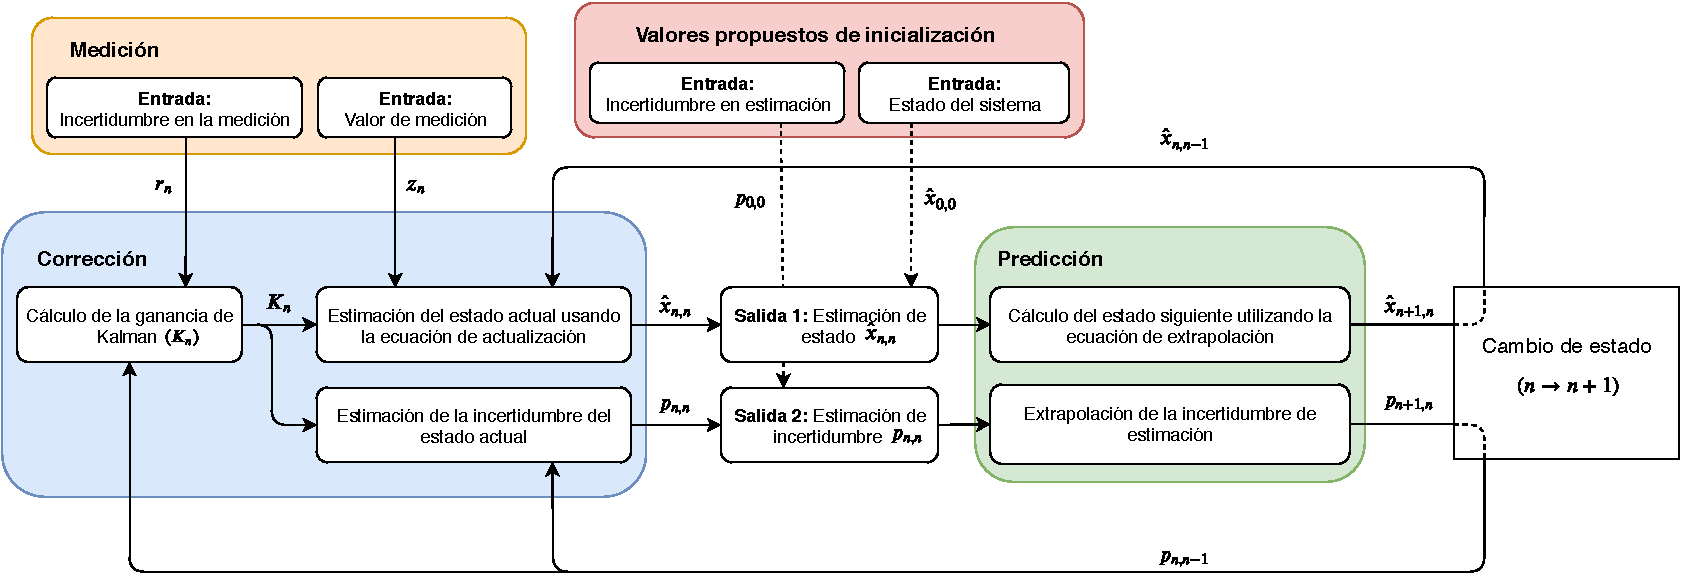
\includegraphics[scale=0.6]{images/kalman_extended_diagram.pdf}
\caption{Diagrama extendidio del funcionamiento paso a paso del Filtro de Kalman}
\label{fig:kalman_extended_diagram}
\end{figure}

		\subsubsection*{Modelado del sistema}
Para desarrollar las ecuaciones de extrapolación de estado se considerará que el balón se desplazará en el suelo sin elevarse o tener rebotes, por lo que el vector de estado $\hat{x}_n$ que describe la estimación de posición y velocidad en el plano \textit{(x, y)} es \ref{eq:state_vector}, siguiendo la nomenclatura que se vio en la sección 2.4.

\begin{equation}
\hat{x}_{n,n} = \begin{bmatrix}
x_1\\ 
y_1\\ 
x_2\\ 
y_2
\end{bmatrix}
\label{eq:state_vector}
\end{equation}

Dado que la única fuerza de entrada en el balón es la fricción, la cual depende del coeficiente de fricción dinámica y la gravedad el vector \textit{û} es representado como:
\begin{equation}
\hat{u}_n = \begin{bmatrix}
F_x\\
F_y
\end{bmatrix} = 
\begin{bmatrix}
0\\
0
\end{bmatrix}
\label{eq:input_signal}
\end{equation}


Como se vio en la sección 2.4, Figura \ref{fig:Kalman_scheme}, la ecuación de extrapolación de estado es:
\begin{equation}
\hat{x}_{n+1,n} = F \hat{x}_{n,n} + G \hat{u}_{n,n} + \omega_n
\label{eq:extrapolation_equation}
\end{equation}

No obstante, con la deducción de la ecuación de posición, el modelo no es lineal, por lo que la ecuación \ref{eq:extrapolation_equation}, usando el Filtro de Kalman Extendido se transforma en:

\begin{equation}
\hat{x}_{n+1,n} = f(\hat{x}_{n,n}, \hat{u}_{n,n}) + \omega_n
\label{eq:efk}
\end{equation}


\ref{eq:state_variable_2} es el modelo en variables de estado, continuo. Para el EKF se discretiza este modelo. Y la señal de entrada F = 0. 

El modelo discreto del sistema con ruido es:
\begin{eqnarray*}
x_{1_{n+1,n}} &=& x_{1_{n,n}} + \Delta t x_{2_{n,n}} + \omega_1\\ %Modelo1
y_{1_{n+1,n}} &=& y_{1_{n,n}} + \Delta t y_{2_{n,n}} + \omega_2\\ %Modelo2
x_{2_{n+1,n}} &=& x_{2_{n,n}} - \Delta t \frac{1}{m}\mu_d m g + \frac{1}{m} F_x + \omega_3\\ %Modelo3
y_{2_{n+1,n}} &=& y_{2_{n,n}} - \Delta t \frac{1}{m}\mu_d m g + \frac{1}{m} F_y + \omega_4 %Modelo4
\end{eqnarray*}

O puesto en forma matricial:

\begin{equation}
\hat{x}_{n+1,n} =
\begin{bmatrix}
1 & 0 & \Delta t & 0\\ 
0 & 1 & 0 & \Delta t\\
0 & 0 & 1 & 0\\
0 & 0 & 0 & 1\\
\end{bmatrix}
\begin{bmatrix}
x_{1_{n,n}}\\ 
y_{1_{n,n}}\\
x_{2_{n,n}}\\
y_{2_{n,n}}
\end{bmatrix}
+
\begin{bmatrix}
0 \\
0 \\
- \Delta t \mu_d g \\
- \Delta t \mu_d g 
\end{bmatrix}
+
\begin{bmatrix}
\omega_1 \\ 
\omega_2 \\
\omega_3 \\
\omega_4
\end{bmatrix}
\end{equation}	

De las cuatro ecuaciones de estado, se miden dos:
\begin{eqnarray*}
z_1 &=& x_1 + v_1\\
z_2 &=& y_1 + v_2\\
z_3 &=& x_2 + v_3\\
z_3 &=& y_2 + v_4
\end{eqnarray*}

o en forma matricial:
\begin{equation}
\hat{z} =
\begin{bmatrix}
x_1 \\ 
y_1\\
x_2\\
y_2
\end{bmatrix}
+
\begin{bmatrix}
v_1 \\ 
v_2\\
v_3\\
v_4
\end{bmatrix}
\end{equation}

$\Omega = [\omega_1, ... \omega_4]$ es un vector de ruido con distribución normal, media cero, y matriz de covarianza $Q\in \mathbb{R}^{4\times 1}$.

		\subsubsection*{Extrapolación de la incertidumbre de estimación}
	El proceso de estimación en el Filtro de Kalman es un modelo basado en la \textit{esperanza} de una serie de variables aleatorias para obtener el valor \textit{oculto} que se considera el real. Este proceso de filtrado considera que todos los errores tanto en medición como en estimación tienen una \textit{distribución gaussiana} por lo que cada incertidumbre tiene que expresarse como la varianza de una recompilación de datos. De una manera análoga a la predicción de posición y velocidad en un tiempo $\Delta t$ la incertidumbre de estimación se puede calcular con las siguientes ecuaciones:

\begin{eqnarray*}
	Px_{1_{n+1,n}} = Px_{1_{n,n}} + \Delta t^{2} Px_{2_{n,n}} + q_{x_1}\\
	Py_{1_{n+1,n}} = Py_{1_{n,n}} + \Delta t^{2} Py_{2_{n,n}} + q_{y_1}\\
	Px_{2_{n+1,n}} = Px_{2_{n,n}} 				    		  + q_{x_2}\\
	Py_{2_{n+1,n}} = Py_{2_{n,n}}							  + q_{y_2}\\
\end{eqnarray*}

O en su forma matricial:

\begin{equation}
\hat{P}_{n+1,n} =
\begin{bmatrix}
1 & 0 & \Delta t^{2} & 0 \\ 
0 & 1 & 0 & \Delta t^{2} \\
0 & 0 & 1 & 0\\
0 & 0 & 0 & 1
\end{bmatrix}
\begin{bmatrix}
Px_{1_{n,n}}\\ 
Py_{1_{n,n}}\\
Px_{2_{n,n}}\\
Py_{2_{n,n}}
\end{bmatrix}
+
\begin{bmatrix}
q_{x_1}\\ 
q_{y_1}\\
q_{x_2}\\
q_{y_2}
\end{bmatrix}
\end{equation}


		\subsubsection*{Obtención de la ganancia de Kalman}
	Una vez teniendo la predicción del estado siguiente, es posible comparar las mediciones con las predicciones préviamente hechas para hacer un proceso de corrección. Para esto es necesario obtener el peso de la ganancia de Kalman que se describe con la siguiente ecuación:
\begin{equation}
	K_n = P_{n,n-1} (P_{n,n-1} + R_n)^{-1}
\end{equation}


		\subsubsection*{Corrección de estimación de estado}
	Con cada nueva medición, se procede a hacer la corrección del estado presente, haciendo uso del la ganancia del filtro para poder \textit{decidir} si es más fiable la medición o la predicción.

\begin{equation}
\hat{x}_{n,n} = \hat{x}_{n,n-1} + K_n(z_n - \hat{x}_{n,n-1})
\end{equation}
	
		\subsubsection*{Corrección del error de covarianza}
	De una manera muy similar el error de covarianza se puede actualizar utilizando la ganancia de Kalman:

\begin{equation}
P_{n,n} = (I - K_n) P_{n,n-1}
\end{equation}

	\section{Obtencion de los parametros}
		\subsection*{Coeficiente de fricción dinámica}
	De acuerdo con la ecuación \ref{eq:position_prediction} y como se vio a lo largo de su deducción, el modelo de la posición del balón respecto al tiempo, depende únicamente del coeficiente de fricción dinámica entre el balón y el material el cual se desplaza. Para obtener dicho coeficiente se optó por la solución más simple, la cual consiste en medir diréctamente la fuerza que se opone al desplazamiento, por medio de un dinamómetro de resorte marca \textit{Pasco} con rango de 0 a 10[N] y una resolución de 0.1[N]. Véase la figura \ref{fig:dynamometer}. 
	
\begin{figure}
\centering
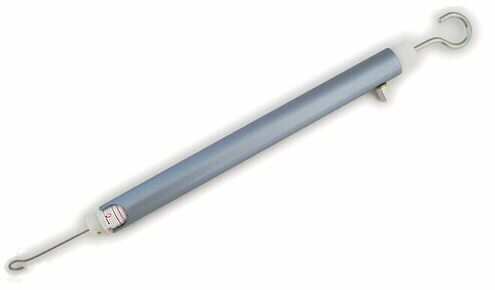
\includegraphics[scale=0.4]{images/dynamometer.jpg}
\caption{Dinamómetro de resorte utilizado para obtener la fuerza de fricción}
\label{fig:dynamometer}
\end{figure}	

	Las medidas del dinamómetro del peso del balón dio $2.2[N]$, de la fuerza de fricción estática $F_{e} = 1.5[N]$ y de la fuerza de fricción dinámica $F_{d} = 0.8[N]$. 

	Por lo que se puede aplicar la segunda ley de Newton (de manera simplificada) para despejar el coeficiente de fricción deseado:
\begin{equation}
F_d = N\mu_d 
\end{equation}
	En donde $N$ es la fuerza normal a la superficie con la misma magnitud del peso del balón (por considerar que se está desplazando de manera horizontal). Por tanto la fuerza de fricción dinámica es:
	
\begin{equation}
	\mu_d = \frac{F_d}{N}
	      = 0.3636		
\end{equation}
	
		\subsection*{Parámetros de Kalman}
		Como en muchos sistemas de control, siempre es mejor variar los parámetros conforme se hagan pruebas, a fin de obtener resultados más óptimos a lo que uno espera. Siendo así, los siguientes parámetros son los que se fueron variando con cada prueba y se decidió que fueron los mejores para filtrar los diversos errores inherentes al sistema. 
		
		\subsubsection*{Vector de ruido del proceso}
\begin{equation}
\Omega = \begin{bmatrix}
0.015	\\ 
0.0\\ 
0.015\\ 
0.0
\end{bmatrix}
\label{eq:process_noise_vector}
\end{equation}

		\subsubsection*{Matriz de covarianza del ruido del proceso}
\begin{equation}
Q = \begin{bmatrix}
0.000001	\\ 
0.0\\ 
0.000001\\ 
0.0
\end{bmatrix}
\label{eq:process_noise_matrix}
\end{equation}

		\subsubsection*{Matriz de error de medición}
\begin{equation}
R_n = \begin{bmatrix}
0.00001	\\ 
0.00001\\ 
0.00001\\ 
0.00001
\end{bmatrix}
\label{eq:noise_measurement}
\end{equation}

		\subsubsection*{Valores iniciales de entrada}
		Debido a que el algoritmo se encarga de converger los valores de entrada con el valor esperado de cada estado, por lo tanto no son de mucha importancia los valores $\hat{x}_{0,0}$ y $\hat{P}_{0,0}$.
\begin{equation}
\hat{x}_{0,0} = \begin{bmatrix}
-0.3\\ 
-0.3\\ 
0.3\\ 
0.3
\end{bmatrix}
\label{eq:initial_state_vector}
\end{equation}

\begin{equation}
P_{0,0} 
=
\begin{bmatrix}
0.1 \\ 
0.1 \\
0.1 \\
0.1 \\
\end{bmatrix}
\label{eq:initial_cov_vector}
\end{equation}	
\chapter{Implementación}

	\section{El robot bípedo Nimbro OP}
	La implementación de los algoritmos de visión artificial está planeada para usarse para el robot bípedo Nimbro OP (Open Platform) que está diseñado para jugar fútbol, en competencias como la RoboCup \textit{Humanoid League} y es compatible con la categoría \textit{TeenSize}.

	\textit{Nimbro-OP} (Figura \ref{fig:Nimbro-OP}) fue el primer prototipo para modular a los humanoides \textit{open-source} para investigación y educación. 
	\subsubsection*{Características de hardware}
	\begin{itemize}
	\item Cuenta con una altura de 95cm y un peso aproximado de 6.6kg.
	\item 20 actuadores interconectados (motores Dynamixel).
		\begin{itemize}
			\item 6 por cada pierna (MX-106)
			\item 3 por cada brazo (MX-64)
			\item 2 en el cuello (MX-64)
		\end{itemize}
	\item PC con doble núcleo (Zotac ZBOX nano XS)
		\begin{itemize}
		\item Procesador AMD E-450(2x1.65GHz) 
		\item 2GB RAM, 64GB SSD
		\item USB 3.0, HDMI, Gigabit Ethernet
		\end{itemize}
	\item WiFi: IEEE 802.11b/g/n
	\item Cámara de amplio ángulo de visión (Logitech C905)
	\item Sensores de inercia (Dentro del controlador Ronotis CM-730)
		\begin{itemize}
		\item Acelerómetro de 3 ejes
		\item Giroscopio de 3 ejes
		\end{itemize}
	\item Batería de Litio de 11.1V a 4.5Ah
	\item Chasis de fibra de carbono, aluminio y ABS plus
	\end{itemize}
	
	\subsubsection*{Características de software}
	\begin{itemize}
	\item El software es compatible tanto para Linux como Windows.
	\item Tiene un desarrollo basado en la plataforma ROS para proporcionar la abstracción de hardware.
	\item Cuenta con software de código abierto que \textit{Robotis} lanzó para DARwin-OP para comportamientos y habilidades básicas en fútbol.
	\end{itemize}
	
\begin{figure}
\centering
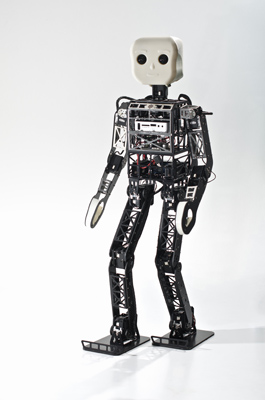
\includegraphics[scale=2.0]{images/Nimbro-OP.jpg}
\caption{Robot humanoide tipo Nimbro-OP}
\label{fig:Nimbro-OP}
\end{figure} 
	
	\section{La bilbioteca OpenCV}
OpenCV (\textit{Open Computer Vision}) es una biblioteca \textit{open source} diseñada para visión computacional. Esta biblioteca está escrita principalmente en C y C$++$ y es capaz de ejecutarse en diversos sistemas operativos, tales como: \textit{Windows}, \textit{Linux}, o \textit{Mac OS X}.

OpenCV fue desarrollada para hacer procesos más eficientes cuando se hace visión con aplicaciones en tiempo real. Una de las metas de OpenCV es proveer una infraestructura sencilla y sofisticada para  diferentes tipos de usuarios, que van desde profesores, estudiantes, profesionistas, desarrolladores, y autodidactas. La librería cuenta con más de 500 funciones que se extienden en diversas áreas de visión, incluyendo inspección en la fabricación de productos, seguridad, calibración de cámaras, visión estéreo, robótica, etc.

	Las principales funciones de OpenCV que se utilizaron para la elaboración de este trabajo fueron:  \textit{cv::calibrateCamera()} para hacer la corrección de las distorsiones (véase la sección 3.2), \textit{cv::cvtColor()} para cambiar del espacio de color RGB al HSV, \textit{cv::InRange()} para realizar la segmentación de color del objeto de interés (véase la sección 3.3), \textit{cv::erode()} y \textit{cv::dilate()} para implementar los operadores morfológicos, junto con \textit{cv::findNonZero()} para obtener el centroide de la figura proyectada en la imagen. 
	
	\section{La plataforma ROS}
		\subsection*{¿Qué es ROS?}
Citando a \cite{pyo2015ros} ROS es un meta sistema operativo \textit{open-source} que provee servicios a las aplicaciones de robótica, servicios que comunmente se esperan de un sistema operativo, tales como: abstracción de hardware, control de dispositivos a \textit{bajo nivel}, paso de mensajes entre procesos, ordenamiento y manejo de distintos tipos de paquetes. ROS también provee herramientas y bibliotecas para obtener, construir, escribir y ejecutar programas a través de multiples computadoras.\\

ROS es la abreviación en inglés de \textit{Robot Operating System} lo cual se prodría traducir al español como Sistema Operativo de Robots. Se podría pensar que ROS es un sistema operativo, sin embargo el término mejor empleado es el de \textit{Meta Sistema Operativo}, y aunque no está definido en el diccionario, se puede describir como un sistema que realiza procesos tales como programación, ejecución, monitoreo, y manejo de errores, utilizando una capa de visualización entre aplicaciones y recursos informáticos distribuidos.\\

Dicho lo anterior, ROS no es un sistema operativo convencional, tal como \textit{Windows}, \textit{Linux}, o \textit{Android}, sino una plataforma que se ejecuta dentro del sistema operativo instalado. A menudo, para utilizar ROS se requiere tener instalado \textit{Ubuntu}, que es un sitema basado en las distribuciones de \textit{Linux}. No obstante, es posible usarse en distintos sitemas, tal y como se muestra la Figura \ref{fig:meta_operating_system}. 
\begin{figure}
\centering
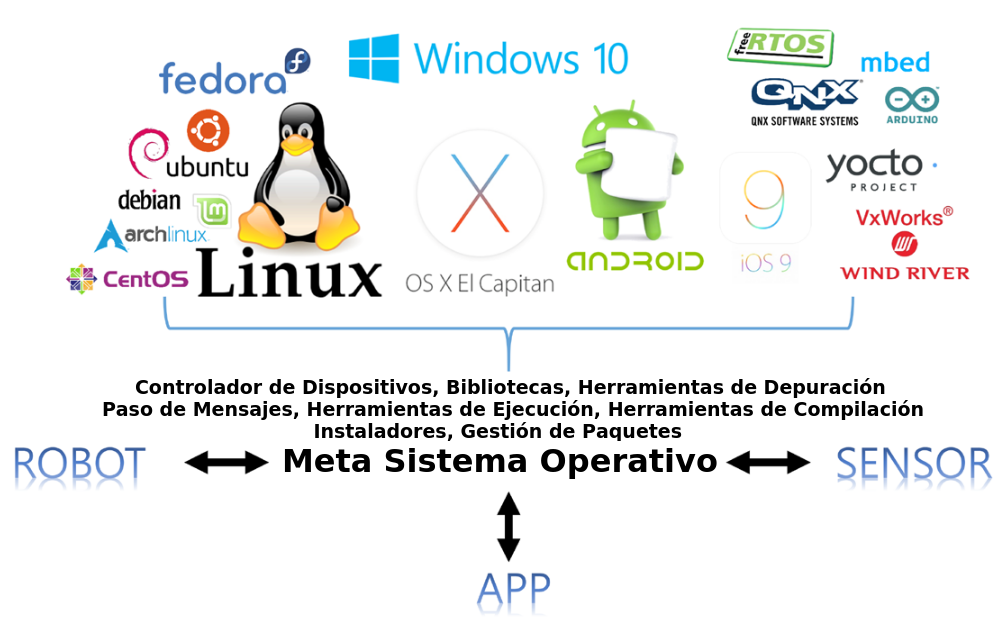
\includegraphics[scale=0.5]{images/meta_operating_system.png}
\caption{Esquema de la abstracción de harware por ROS en distintos Systemas Operativos}
\label{fig:meta_operating_system}
\end{figure} 

		\subsection*{Objetivos al utilizar ROS}
Aunque existen diversas plataformas de robótica (OpenRTM, OPRoS, Player, Orca, Microsoft Robotics Studio, etc.), ROS está orientado a construir entornos de desarrollo para software de robótica a un nivel global, con esto se espera que el código de diferentes desarrolladores se pueda usar, modificar o mejorar para hacer crecer el entorno mismo, es por eso que posee las siguientes características:

\begin{itemize}
\item \textbf{Distribución de procesos:}
Están programados en unidades mínimas de procesamiento (nodos). Cada uno de estos procesos se ejecuta de manera independiente y es capaz de intercambiar datos con otros de manera sistemática.  
\item \textbf{Manejo de paqueterías:}
Cuando varios procesos tienen propósitos similares, estos se manejan dentro de un \textit{paquete} que haga los procesos más ordenados y fáciles de desarrollar.
\item \textbf{Repositorios públicos:}
Cada paquete se hace público dentro de un repositorio (por ejemplo GitHub) para que la comunidad de desarrolladores puedan acceder a él. 
\item \textbf{API (Interfaz de Programación de Aplicaciones):}
Cuando se desarrolla un programa en ROS, generalmente se llaman funciones ya existentes fácilmente insertarlas dentro del código que se esté construyendo.
\item \textbf{Soporte de distintos lenguajes de programación:}
La plataforma ROS posee una \textit{bilioteca de clientes} para facilitar el trabajo de los programadores. La biblioteca puede importar lenguajes de programación que son bastantes populares, tales como Python, C$++$, Java, Ruby, Lips, entre otros.
\end{itemize}
		\subsection*{Breve historia de ROS}
\textit{Robot Operating System} fue creado en Mayo del 2007 dentro del \textit{Standford Artificial Intelligence Laboratory}. Se podría decir que el predecesor de ROS es un proyecto llamado \textit{SwitchYard}, el cual es un software creado para el desarrollo de inteligencia artificial de robots.

En noviembre del 2007 la compañía estadounidense \textit{Willow Garage} empezó el desarrollo de ROS dentro del campo de los robots de servicio. De esta manera ROS vino al mundo oficialmente el 22 de Enero del 2010 con la versión llamada \textit{ROS 1.0}, sin embargo la versión más conocida fue \textit{Box Turtle} lanzada en Marzo del mismo año.

La plataforma ROS es actualizada cada dos años (entre el lapso de Abril-Octubre), lo que significa que cada versión tiene soporte durante aproximadamente cinco años. Para propósitos de esta tesis se optó por utilizar la versión \textit{ROS-Melodic} instalado en Ubuntu 18.04 \textit{Bionic Beaver (LTS)}.

	\section{Integración de los diferentes programas}
	Para hacer uso del humanoide se requiere clonar un repositorio que se encuentra en la siguiente liga: https://github.com/mnegretev/Humanoids . Este repositorio contiene distintos programas, unos para que el hardware del humanoide se pueda comunicar con un ordenador, otros para el procesamiento de datos, concernientes a las entradas de sensores y control de actuadores e incluso para hacer pruebas remotas con el simulador.
	
	Debido a las circunstancias extraordinarias dadas por la pandemia del coronavirus, el distanciamiento social dificultó la realización de pruebas con el robot físico, por lo que se optó por seguir el desarrollo de software de la parte simulada. Haciendo el software los suficientemente robusto para que sea capaz de usarse tanto en el robot real como en el simulado.
	
	Aunque actualmente no se puedan hacer pruebas con el robot en físico, trabajar con la parte simulada del humanoide representa claras ventajas, las cuales son: 
	 
	\begin{itemize}
	 	\item Complementar el simulador con plug-ins y herramientas extra para la simulación de una cámara virtual dentro del simulador Gazebo.
	 	\item Control del ruido inherente a la medición de los sistemas, ya que se puede probar la robustez del algoritmo de filtrado con diferentes niveles de ruido.
	 	\item Desarrollo del código para el simulador, para su aprendizaje y complementación de la documentación.
	 	\item Hacer el software más disponible para desarrolladores que no tengan la posibilidad de interactuar con el robot o que se encuentren en lugares distantes.
	 	\item Evitar retrazos por fallas del hardware.
	\end{itemize}
	
		\subsection*{Descripción de los principales nodos usados en este trabajo}
		El repositorio anteriormente mencionado tiene instrucciones para la instalación del entorno de trabajo y corrimento de los programas. Para probar el simulador, el comando de inicio es: $$roslaunch surge_-et_-ambula humanoid_-simul.launch$$ 

		Éste es un comando que levanta distintos nodos que se comunican entre sí para simular las variables físicas simuladas del robot. Cuando se levanta se puede observar que se abren algunas ventanas, las cuales son del visualizador del robot \textit{Rviz}, el simulador con variables físicas \textit{Gazebo}, una GUI (Graphical User Interface) para manipular las articulaciones del robot y una ventana que simula la imagen obtenida de la cámara simulada. Tal y como se observa en la Figura \ref{fig:gazebo}.
		
\begin{figure}
	\centering
	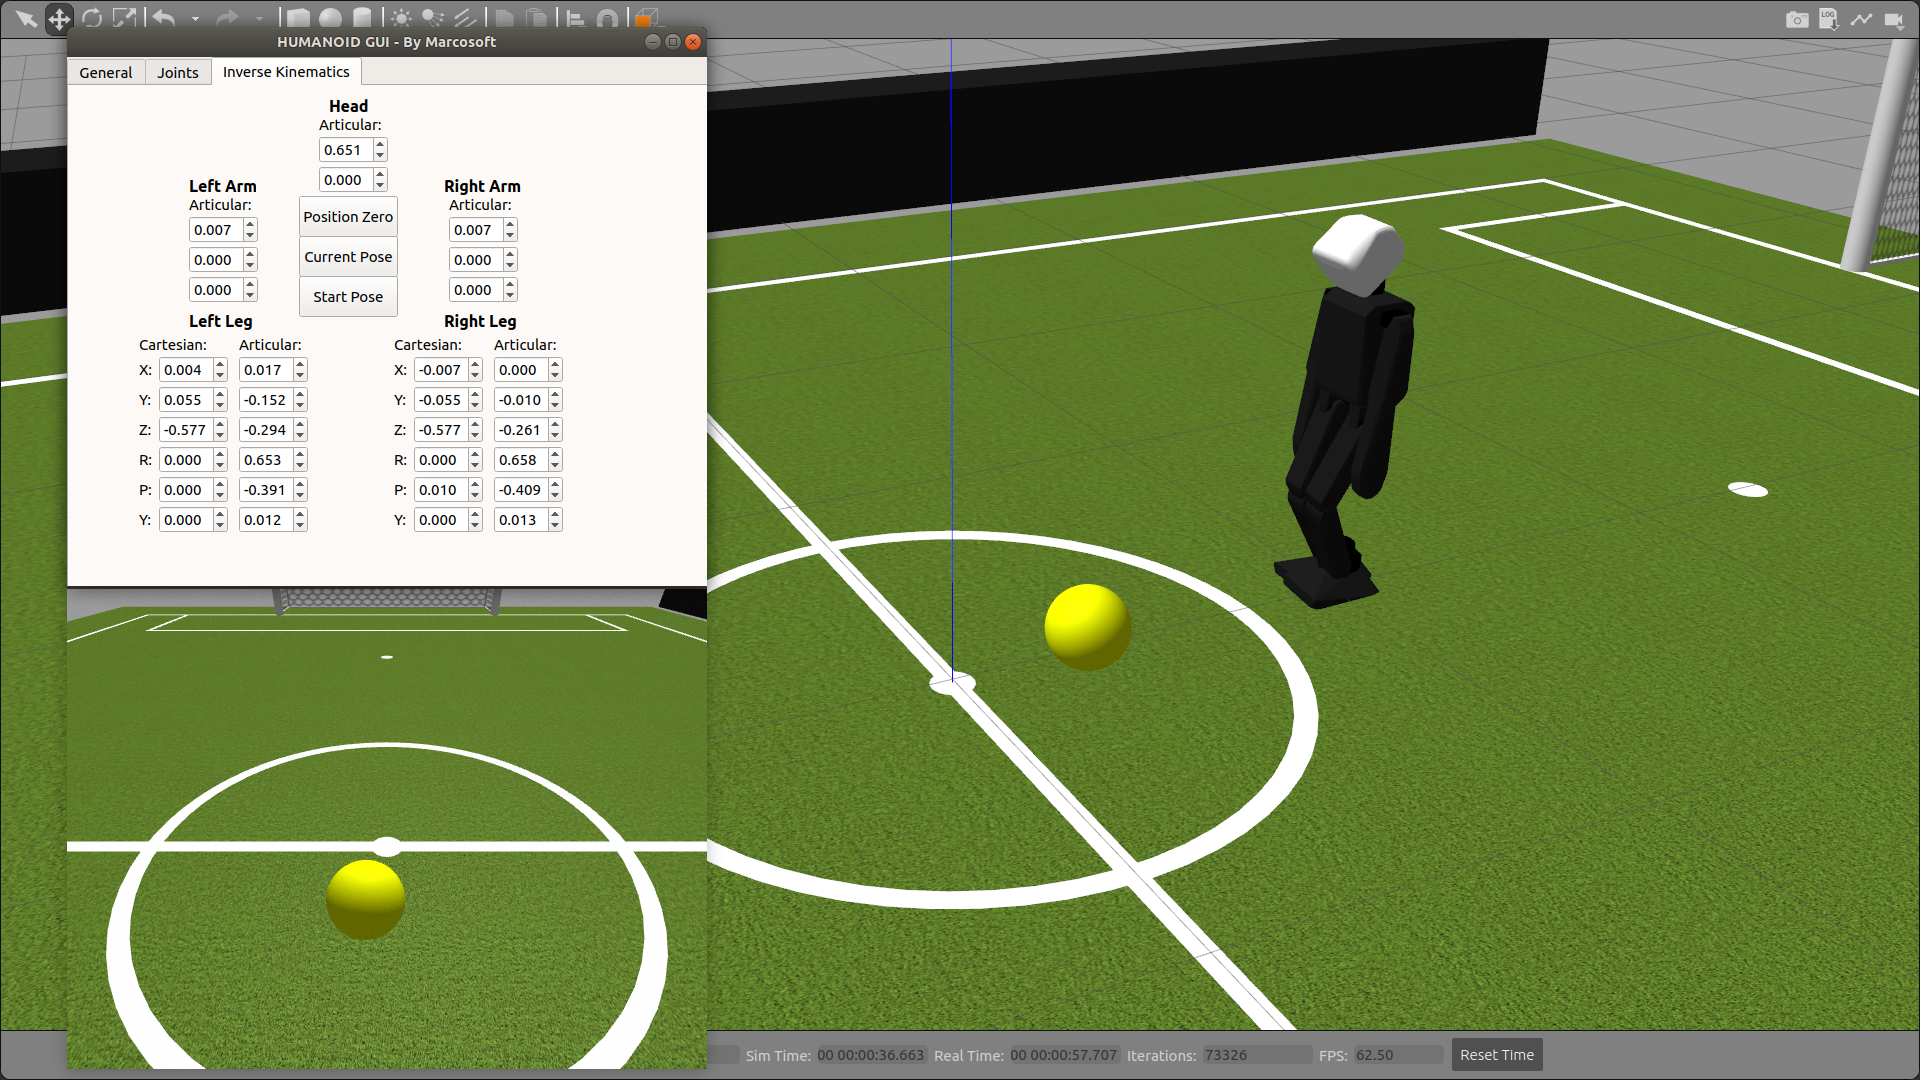
\includegraphics[scale=0.2]{images/gazebo.png}
	\caption{Simulador Gazebo para el humanoide.}
	\label{fig:gazebo}
\end{figure} 
		
			\subsubsection*{Nodo segmentador de color}
			Ejecutando el comando \textit{rosrun $ball_-tracker$ $ball_-tracker_-simul$} se alza el nodo que se subscribe a los tópicos que contienen la información de la imagen RGB obtenida por la cámara. Con esa información se procesa la imagen para segmentar un color deseado guardando los parámetro HSV en un archivo .xml.
			
			\subsubsection*{Nodo que calcula la posición relativa del balón}
			El nodo más importante de esta tesis es el que calcula la posición relativa del balón, ya que de éste depende la precisión y confiabilidad de las mediciones. Con el comando \textit{rosrun $ball_-position$ $ball_-position_-simul$} se levanta, se subscribe a los tópicos de la imagen y hace la segmentación del objeto de interés con base en la teoría vista en el capítulo 3. 
			
			Teniendo ya procesada la sementación, el punto de interés de la figura segmentada es el centroide, con el cual se hacen cálculos geométricos para el posicionamiento del balón, haciendo uso de las herramientas \textit{tf} para conocer la posición y orientación relativa de la cámara con respecto a los pies del robot. Como se ilustra en la Figura \ref{fig:tf}.
			
\begin{figure}
	\centering
	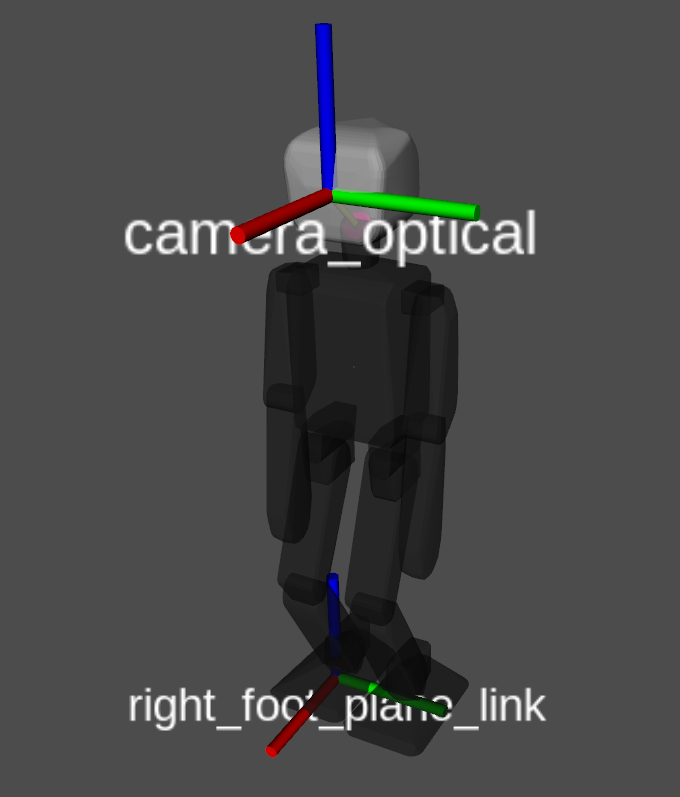
\includegraphics[scale=0.3]{images/tf.png}
	\caption{tf, herramienta de ROS para obtener la información relativa de las articulaciones de un robot (posición y orientación)}
	\label{fig:tf}
\end{figure}
	
			Al procesar la información de posición, el nodo $ball_-position_-simul$ publica un tópico que contiene la posición $x$ y $y$ del balón, por lo que otros nodos pueden hacer uso de esa información.
			
			\subsubsection*{Nodo estimador de posición y velocidad utilizando el Filtro de Kalman Extendido}
			El nodo llamado $kalman_-estimator$ es un \textit{script} escrito en el lenguaje Python, el cual se subscribe a los tópicos de posición del balón para saber la posición instantánea del balón en los ejes $x$ y $y$. Con esto, el programa usa los parámetros de Kalman (véase la sección 4.3) para obtener una correción del ruido y hacer la debida predicción de posiciones y velocidades tomando una determinada cantidad de muestras con una frecuecia aproximada de 30 Hz. Para entender este nodo de una manera más visual la Figura \ref{fig:kalman_flux_diagram} muestra el diagrama de flujo de los principales procesos. 
			
			Se puede revisar el código de este nodo en el \textbf{Apéndice A}.
	Adicionalmente a este programa, hay un código escrito en python para hacer la comparación de la posición real, la medida y la estimación mediante una gráfica, éste no es un nodo sino simplemente un \textit{script} llamado $graph_-kalman_-estimator.py$.
			
			\subsubsection*{Nodo para movimiento del balón}
			Ejecutando en una nueva terminal el comando \textit{rosrun $ball_-position$ $move_-ball_-node$} se inicializa un nodo que mueve el balón simulado a una dirección y velocidad inicial determinada, con base el lo que se vio en la sección 4.2. 
			
			\subsubsection*{Nodo para la secuencia de pateo} 
			El programa que ejecuta el nodo \textit{$ready_-2_-kick$} utiliza la clase Humanoid para hacer movimientos con posiciones predefinidas, en este caso pausandolas para mantenerse parado sobre un pie esperando a que el nodo $kalman_-estimator$ le de la señal para que patee el balón.
		
		
\begin{figure}
	\centering
	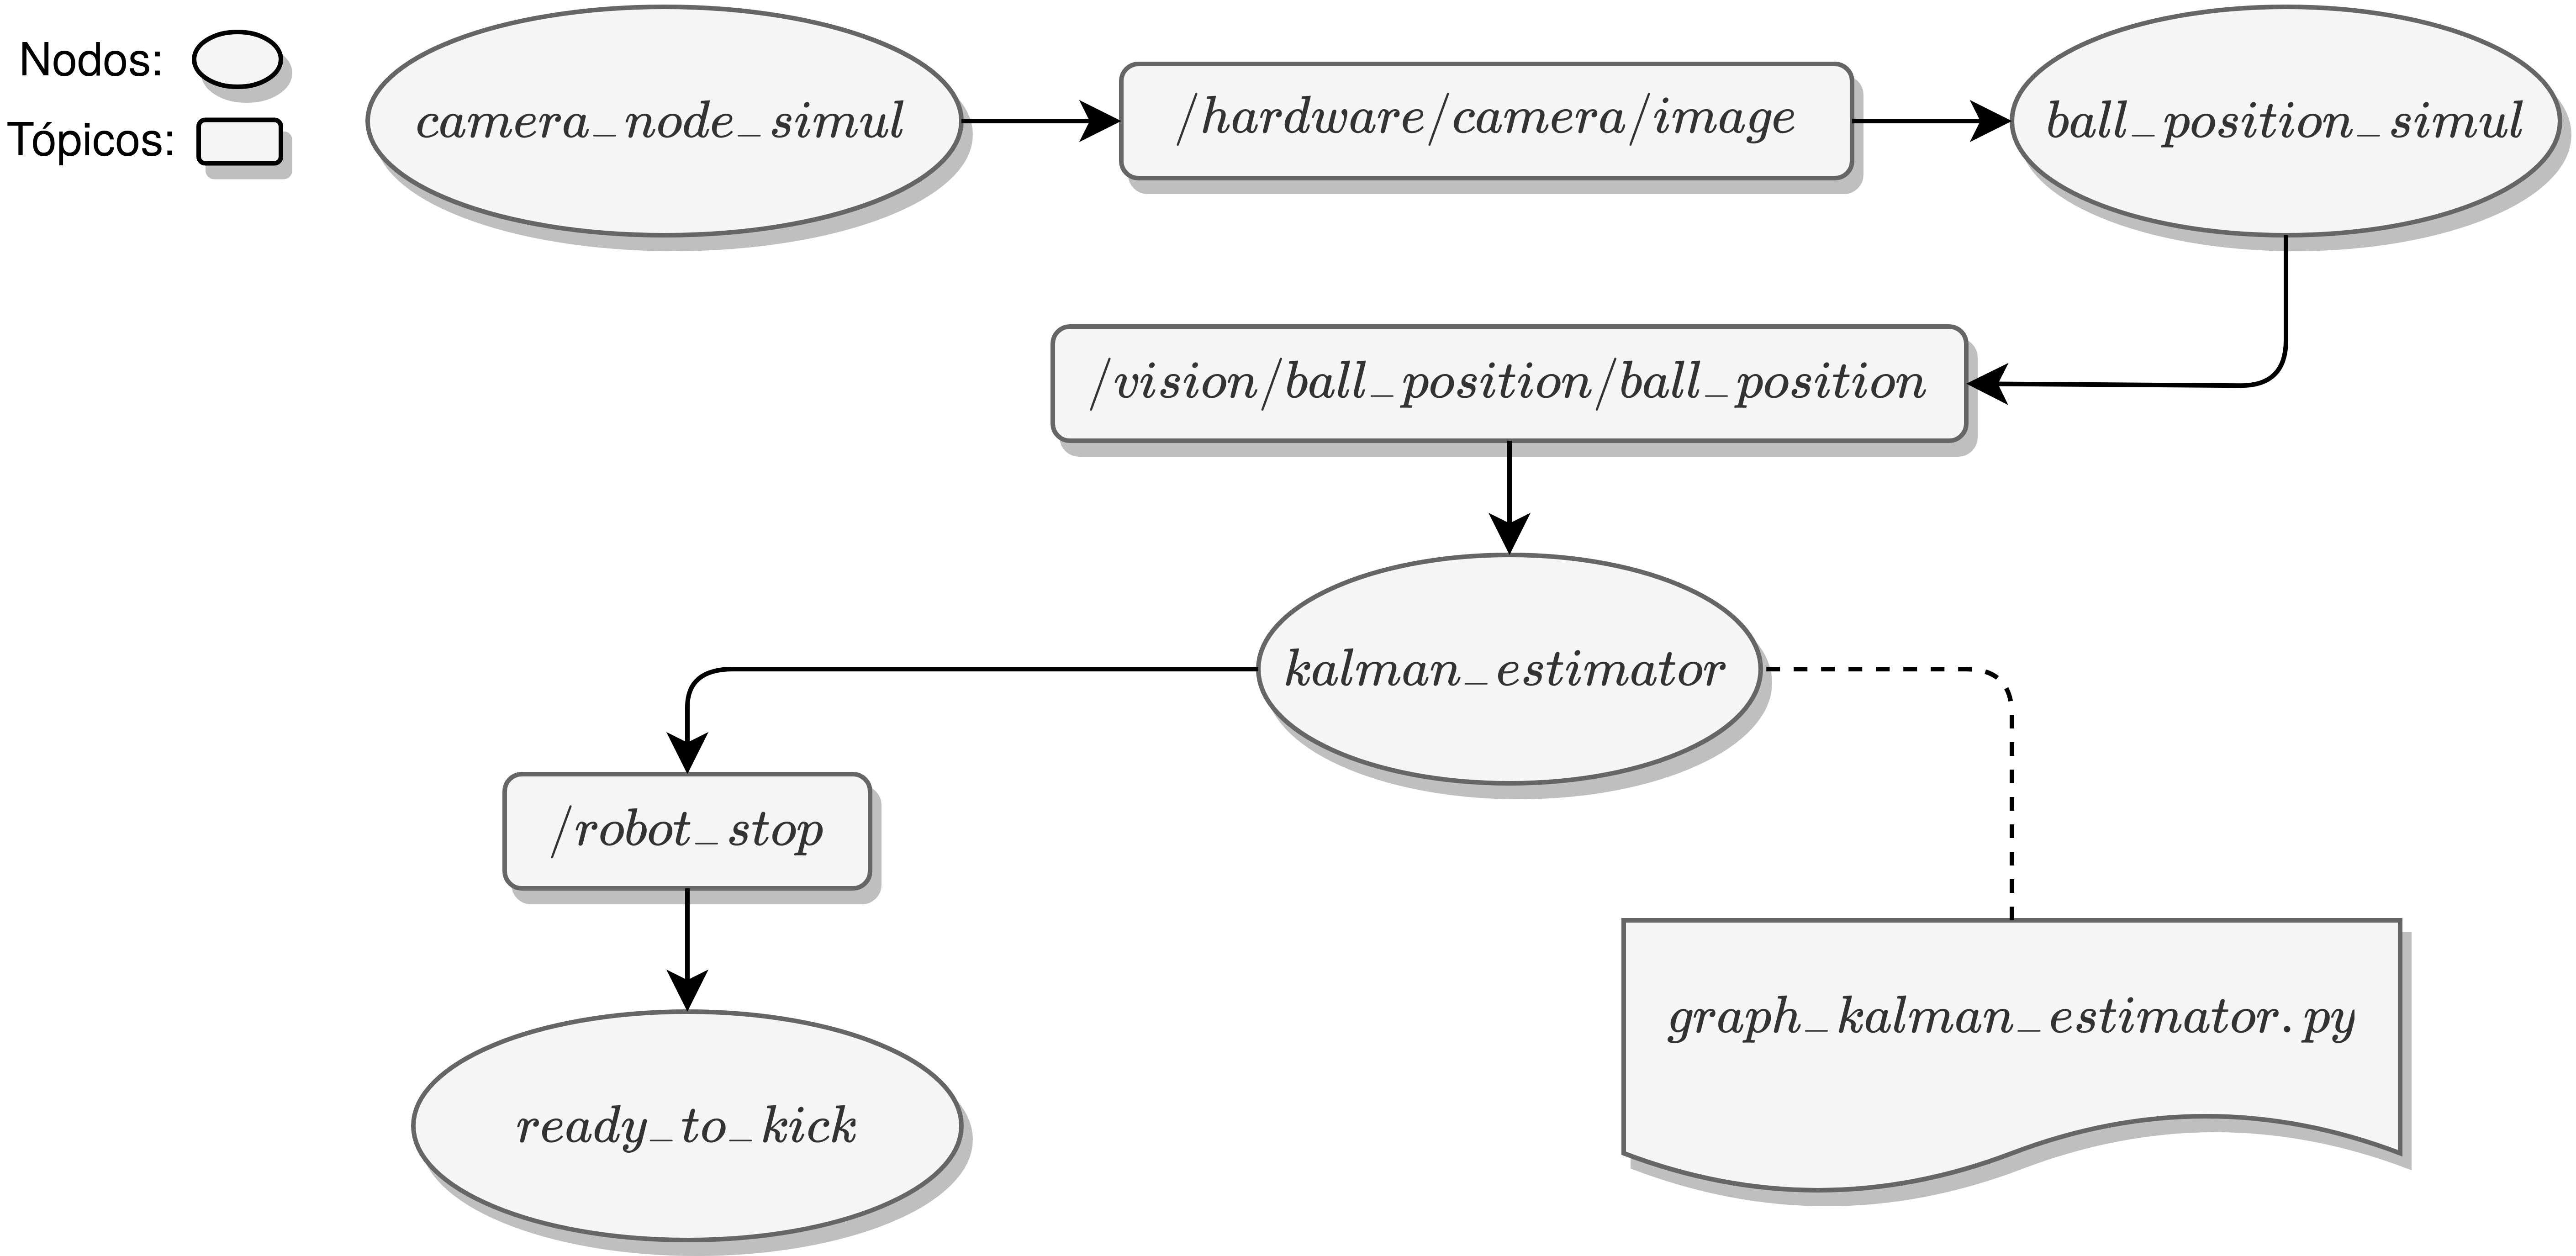
\includegraphics[scale=0.071]{images/nodes_diagram.png}
	\caption{Diagrama simplificado de los principales nodos empleados}
	\label{fig:nodes_diagram}
\end{figure}
		
\begin{figure}
	\centering
	
\includegraphics[scale=0.055]{images/kalman_flux_diagram.png}
	\caption{Diagrama de flujo del nodo estimador de posición y velocidad}
	\label{fig:kalman_flux_diagram}
\end{figure}

		
		
		
	
\chapter{Resultados}
\section{Pruebas de estimación de posición}
\section{Pruebas de estimación de velocidad}
\section{Pateo de un balón como prueba del sistema completo}
\chapter{Discusión}
\section{Conclusiones}
	En este trabajo se fueron integrando conocimientos adquidridos de diversas ramas del conocimiento y materias que se imparten desde los inicios de la carrera de Ingeniería en Mecatrónica, tales como Cálculo Diferencial e Integral, Geometría Analítica, Álgebra Lineal, Cinemática, Ecuaciones Diferenciales, Estadística, Fundamentos de Programación y Programación Orientada a Objetos, Control Automático, Robótica y sobre todo Construcción de Robots Móviles.
	
	Con respecto a la parte de resultados, se puede concluir que los objetivos planteados en esta tesis se cumplieron satisfactoriamente en cuanto al desarrollo del sistema de visión del humanoide (tanto el real como el simulado), el algoritmo de pateo con un control a lazo abierto basado en posiciones predefinidas y en la aplicación del Filtro de Kalman Extendido para la filtración del ruido inherente a las mediciones.
	Al momento de unir los distintos programas en el sistema embebido se presentaron algunos retos a cumplir en cuanto a la optimización de los procesos su debida interconección, para lo cual las herramientas de la plataforma ROS fueron de vital importancia y ayudaron para integrar nodos escritos en diferentes lenguajes de programación.

	En cuanto al objetivo general, se logró cumplir que el robot simulado pateara el balón con una previa predicción de posición. No obstante, por las dificultades causadas por la pandemia, quedará en espera el hacer pruebas con el robot real, con la expectativa de que se requieran sólo cambios mínimos concernientes al hardware y al ruido de medición con variables reales.
	
	Como se vio en la parte de resultados el rango de velocidades del balón tuvo un umbral de 2.0 a 2.8 m/s aproximádamente, por lo que puede decirse que es un rango algo pequeño, y cuando se implemente en el mundo real puede disminuir dependiendo las variaciones del coeficiente de fricción. Una manera en que se podría mejorar lo anterior es adaptando una cámara con mayor rango de visión horizontalmente con las ya conocidas cámaras de \textit{ojo de pezcado}, de esta manera podría tomar las ocho muestras de información para que al estimador le dé tiempo de hacer una estimación con mayor tiempo y distancia.
	
	Una de las ventajas de hacer las pruebas del robot simulado, que al mismo tiempo es una desventaja para el robot real, es el del tiempo de latencia que hay entre la comunicación con la computadora con el hardware del humanoide, es importante de mencionar debido a que representaría un retardo de tiempo a considerar desde que se manda un mensaje hasta que el hardware lo reciba. 
	
	Alguna de las mejoras que se le podrían hacer al algoritmo de pateo es mejorar su estabilidad en cada movimiento, implementandole a un sistema de control de velocidad (ya que sólo cuenta control de posición en cada articulación). A parte de esto sería muy conveniente que se hiciera un control de posiciones con realimentación, ya que es fácil que el robot caiga con cada prueba. Con un sistema a lazo cerrado se obtendría la estabilidad necesaria e incluso se podrían realizar movimientos más rápidos, ampliando sin duda el rango de velocidades a los que el robot pueda patear un balón en movimiento. 
\section{Trabajo Futuro}
	Podría decirse que en este trabajo se desarrolló un sistema de visión de predicción de posición análogo al del ser humano utilizando un método basado en la esperanza de una serie de datos y un previo modelo matemático. Empero esta no es la única forma de emular este tipo de funciones, para futuras propuestas de proyectos, se podría implementar un sistema de estimación basado el redes neuronales o algoritmos genéticos, los cuales no tendrían las mismas limitantes que el Filtro de Kalman, como por ejemplo que se tenga que conocer el coeficiente de fricción dinámica, que se requiera una superficie completamente plana u horizontal y que el balón no tenga rebotes o elevaciones de ningún tipo en cuanto a su trayectoria.

\appendix
\section{Apéndice A: Código del estimador utilizando el Filtro de Kalman Extendido}
\lstinputlisting[language=Python]{kalman_estimator.py}
\begin{appendices}
\chapter{Código del estimador de Kalman}
\lstinputlisting[language=Python]{kalman_estimator.py}
\end{appendices}

%\appendix


\bibliography{References}
\end{document}
